\status{started}
\chapter{MEG II and the Cockcroft–Walton}
\begin{refsection}
{\itshape This Chapter is dedicated to an in-depth description of the MEG search and the MEG II apparatus. After the description of the different subdetectors and their functionality a description of the beamlines will follow. MEG II is served by the main muon beamline, part of the PSI beamlines described in the Introduction Chapter, and a secondary proton beamline equipped with its own Cockcroft–Walton. This machine has different uses in the collaboration, which will be here discussed, and its functioning has been one of my main tasks. For this reason, some additional details will be here included.}

\section{MEG II}
\section{XEC}
    \subsection{Xe scintillation}
    \subsection{Xe as calorimeter}
    \subsection{Cryogenics}
    \subsection{PMTs}
    \subsection{Performances}
    \subsection{LED Calibration}
    \label{LED}

\section{Spectrometer}
    \subsection{COBRA}
    \label{MEG:COBRA}
    \subsection{CDCH}
    \subsection{TC}

\section{Trigger and DAQ}

\status{started}
\section{Beam and target}
    The beam lines at PSI were described in \ref{intro:beamlines}. 
    In particular, the beam line delivering $\mu^+$ to MEG II is the $\pi E5$ line. 
    This line is shown in  Fig. \ref{fig:pie5} and the key elements are here discussed

    \status{started}
    \subsection{$\pi e5$}
        This beam-line has actually two possible configurations: this will allow to share it between MEG II and Mu3e. 
        As already illustrated, the surface muons delivered by this beam-line are produced for the decay of the pions generated as secondary beams from the HIPA proton beam.
        On top of muons, pions and positrons also are transported by the beamline: the rate of the different species is momentum dependent and is shown in Fig.~\ref{fig:pie5:rates}.
        The peak at \SI{29}{MeV/c} is the working point of the experiment.
        \begin{equation}
            \Delta R = a \left\{
                \left[  
                    \left( \frac{200 m_e}{M}\right)^{1/2} f \frac{E}{Mc^2}
                \right]^2 + 
                \left( 3.5\frac{\Delta p }{p}\right)^2
            \right\} ^{1/2} p^{3.5}
        \end{equation}
        The elements that makeup one of the two configurations, the "L" channel, were designed \textit{ad hoc} for MEG II.

        \begin{figure}
            \centering
            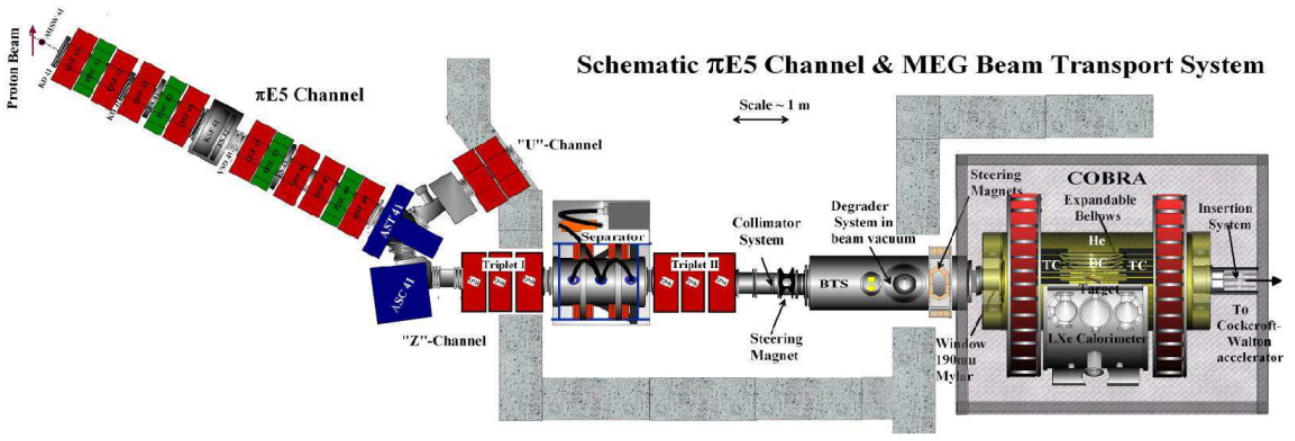
\includegraphics[width = \textwidth]{Figures/MEG/pie5_beamline.png}
            \caption{Detail of the $\pi E5$ beamline at PSI. OLD}
            \label{fig:pie5}
        \end{figure}

        \paragraph{Quadrupoles and separator}
        \paragraph{BTS}
        \paragraph{COBRA} Finally the beam enters COBRA. 
        The design choice for this element was previously illustrated (\ref{MEG:COBRA}). 
        The behavior of the beam inside this element is quite tricky to simulate consistently.
        
    \status{started}
    \subsection{Simulations}
        \paragraph{\gfb}
        \paragraph{\madx} During 2022/2023 Luca Biasia, a Master student in Pisa, developed a \madx\footnote{\madx is a general-purpose tool for charged-particle optics design and can be found \href{http://madx.web.cern.ch/madx/}{\underline{here}}.} simulation to describe the $\pi E5$ line and cross-validate the results obtained using \gfb. 
        My contribution to this simulation was only partial: I provided Luca with some working \madx examples, developed while attending the JUAS, for him to start playing with this simulation framework. 
        After this initial `starting kit', Giovanni Dal Maso was the one overseeing the development while I only followed the updates and gave feedback or suggestions. \\
        After a comparison with data and \gfb some discrepancies arose and, after many iterations, they were associated with the description of the fringing fields of the components in \madx. 
        The solution adopted was to slice the field maps in thin layers and define many thin `\madx elements'. 
        A comparison of the results from QSK41 to COBRA center is shown in Fig.~\ref{fig:madx_vs_g4b}.
        During the beam tuning in June 2023, this simulation was crosschecked: after measuring the beam spot at COBRA center the currents of the magnets were chosen with \madx to obtain a different beam shape. 
        The measurement was consistent with the resulting simulation.
        This was a great achievement and, moving forward, this tool is going to play a key role during the beam tuning.

        \begin{figure}
            \centering
            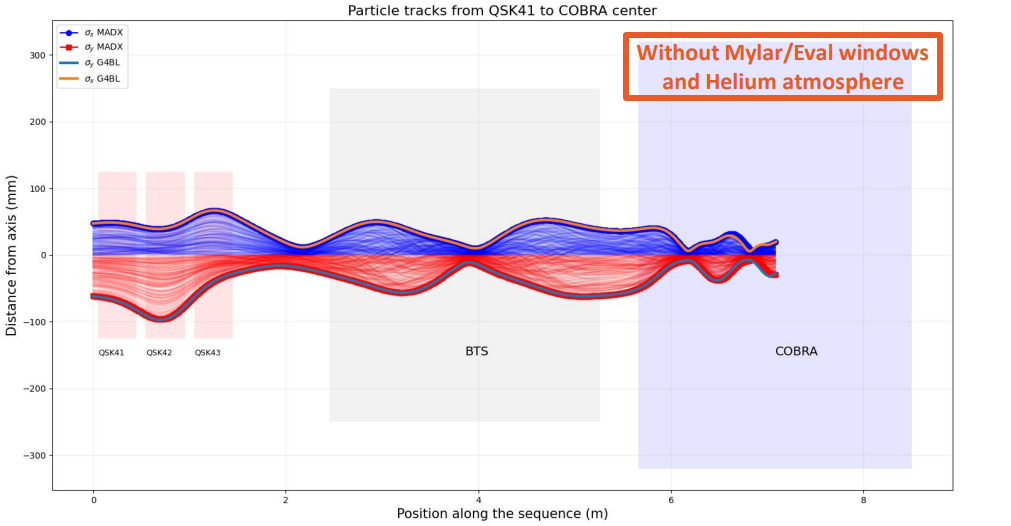
\includegraphics[width = \textwidth]{Figures/MEG/madx_vs_g4b.png}
            \caption{Comperison of the results from the \gfb and \madx simulations for $\pi E5$. While the agreement is very good for most of the beamline, there is some difference inside cobra. This is due to the difficulty in describing the highly `non standard' magnet. Given \madx has no particle interaction, the comparison is fair only when removing all  materials from the beamline in the \gfb simulation.}
            \label{fig:madx_vs_g4b}
        \end{figure}
    
    \subsection{MEG II target}
        \paragraph{Deformation and pictures}

\status{started}
\section{Cockcroft–Walton}
    \label{sec:cw:calib}
    In addition to the muon beamline, MEG II has a Cockcroft–Walton proton accelerator. 
    After the description of the machine, we will see the use of this accelerator by the collaboration: calibrations of the Liquid Xe Calorimeter and exotic searches. 

    \status{review}
    \subsection{Description of the machine}
        \label{sec:cw:machine}
        The accelerator is a single-stage in-line singletron produced by HVEE. 
        This machine is a compact Cockcroft–Walton with a terminal voltage of $0.1\divisionsymbol1.0$ MV and a proton current up to \SI{100}{mA}.
        
        \paragraph{Source} The RF ion source is a bottle of gas that is excited by an RF oscillator. 
        The electrons in the gas are excited and, because of the collisions with the neutral gas particles, cause ionization.
        The plasma produced is confined with an axial magnetic field and serves as the source of positive ions, which are extracted by applying a DC electric field.
        A schematic of the working principle of the RF ion source is shown in Fig.~\ref{fig:CW:sketch:ionsource}

       \begin{figure}
            \centering
            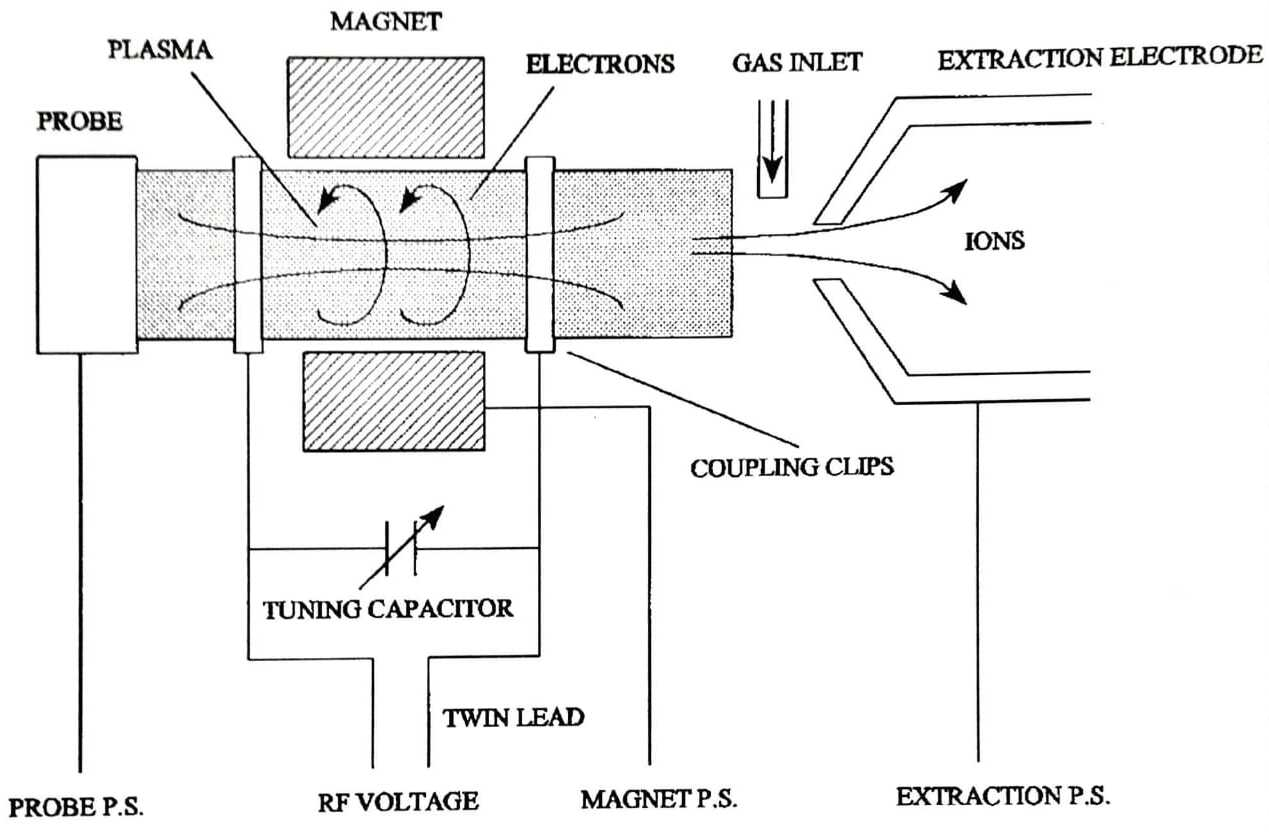
\includegraphics[width=0.8\textwidth]{Figures/MEG/CW/cw_ionsource.jpeg}
            \caption{Sketch of the ion source of the CW.}
            \label{fig:CW:sketch:ionsource}
        \end{figure}
        
        \paragraph{CW-Circuit}
        The high-voltage multiplier and rectifier stack, together with the RF driver and HV control and stabilizing system, is one of the core sections of the machine.
        It is located in the main pressure tank, while the RF resonance coils are in a separate \ce{SF6} filled tank and the RF driver in a separate cabinet.
        This gas is often used as a gaseous dielectric medium because of its high dielectric strength, the result of the gas's high electronegativity
        \footnote{Electronegativity is a measure of the attraction of an atom for bonding electrons in molecules compared to that of other atoms: large values indicate a stronger attraction and it increases from left to right across the periodic table.} and density.
        In the case of an arc, \ce{SF6} can break down in different ways but most of the decomposition products tend to quickly re-form \ce{SF6}, a process termed \textit{self-healing}. 
        Arcing or corona can also produce disulfur decafluoride (\ce{S2F10}), a highly toxic gas, which is the reason extra care is needed when opening such a system.
        This stack is a parallel-fed CW power supply that consists of a series of high voltage rectifiers and capacitive coupling \textit{corona} rings.
        The power is fed via an RF driver capacitive coupled.
        A sketch of the inner structure of a rectifier assembly (\textit{ass'y}) is shown in Fig.~\ref{fig:CW:sketch:rectifier} while in Fig.~\ref{fig:CW:removal} is clearly visible the way the ass'ys are mounted.

        \begin{figure}[ht]   
            \centering
            \subfloat[Schematic of power supply.]{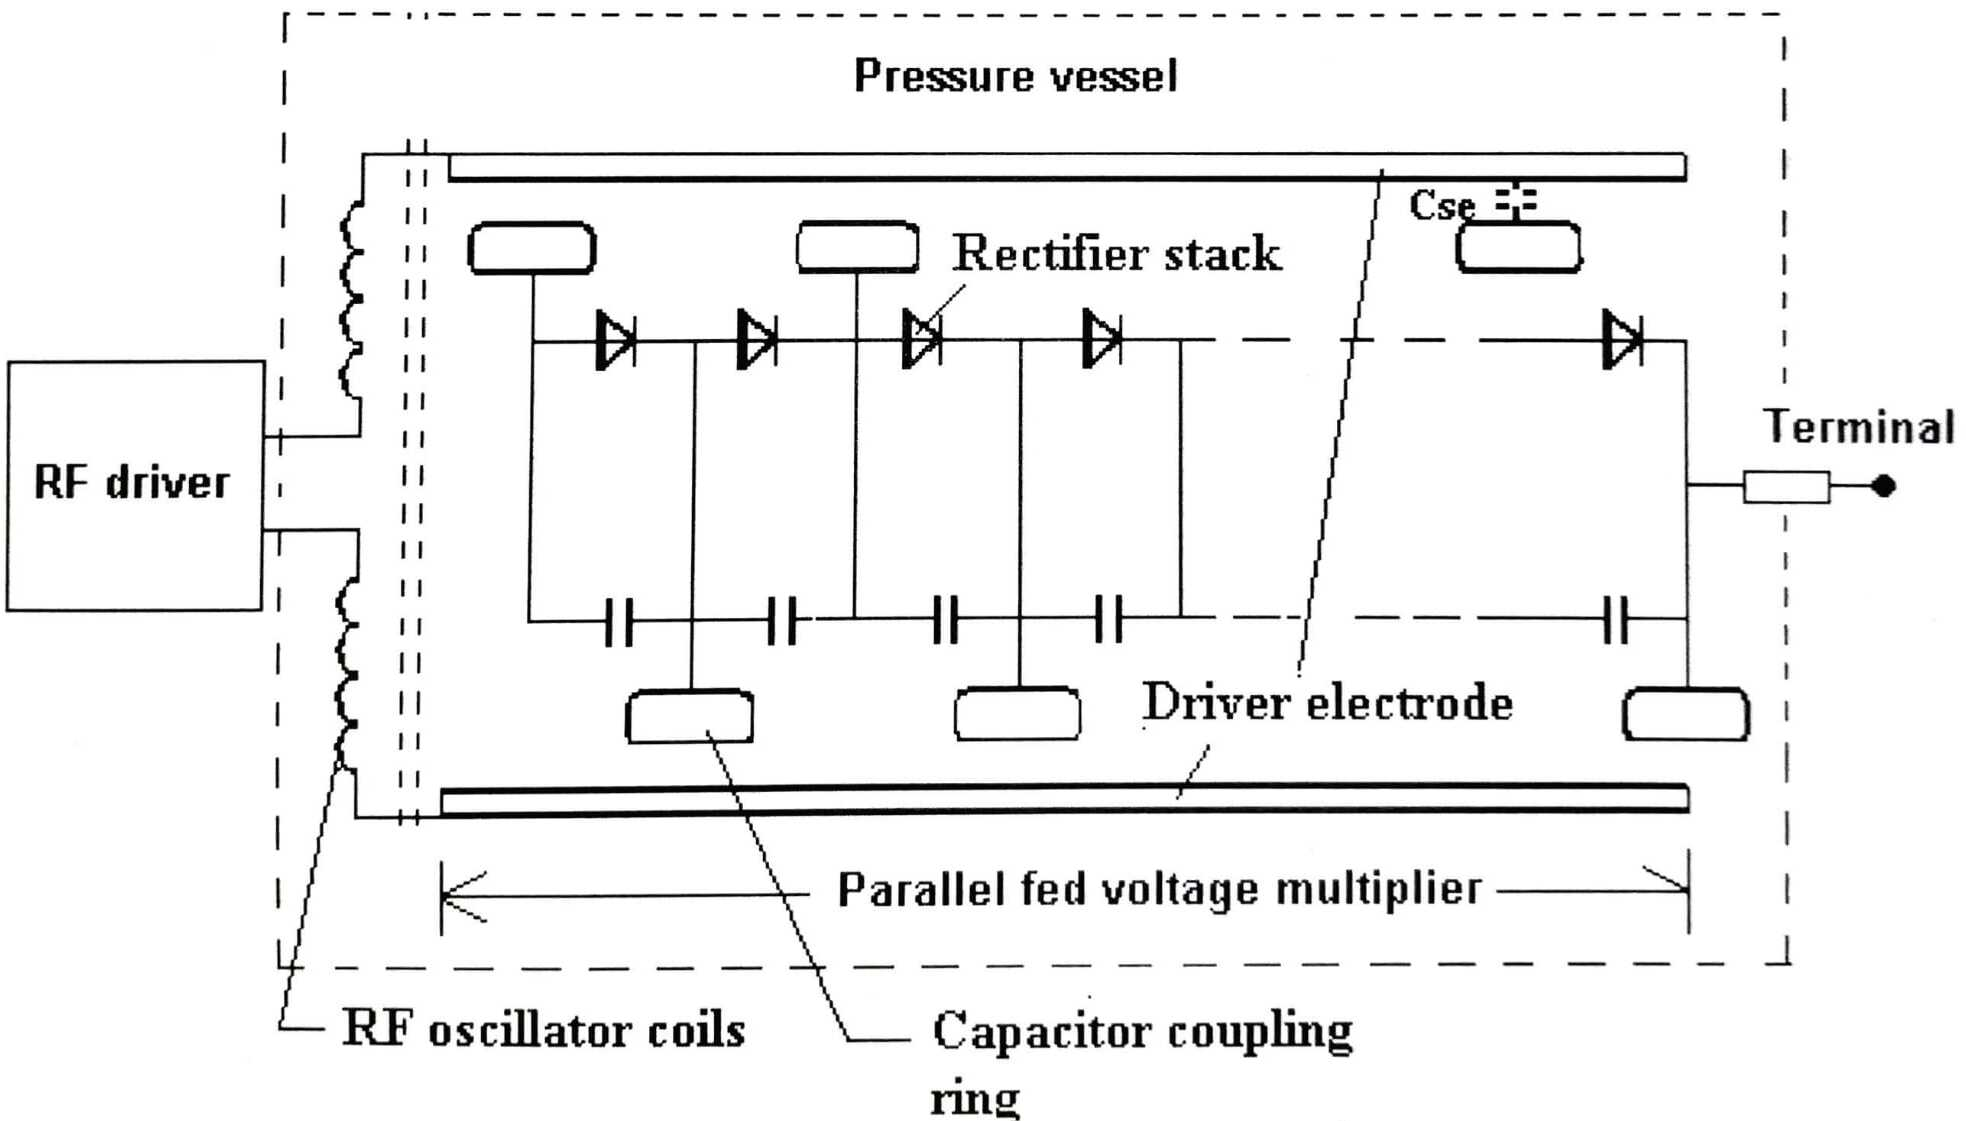
\includegraphics[width=0.8\textwidth]{Figures/MEG/CW/cw_circuit_stack.jpeg}\label{fig:CW:circuit:stack}}\\
            \subfloat[Sketch of the inner structure of a \textit{stack ass'y}: 15 rectifiers and 2 resistors.]{            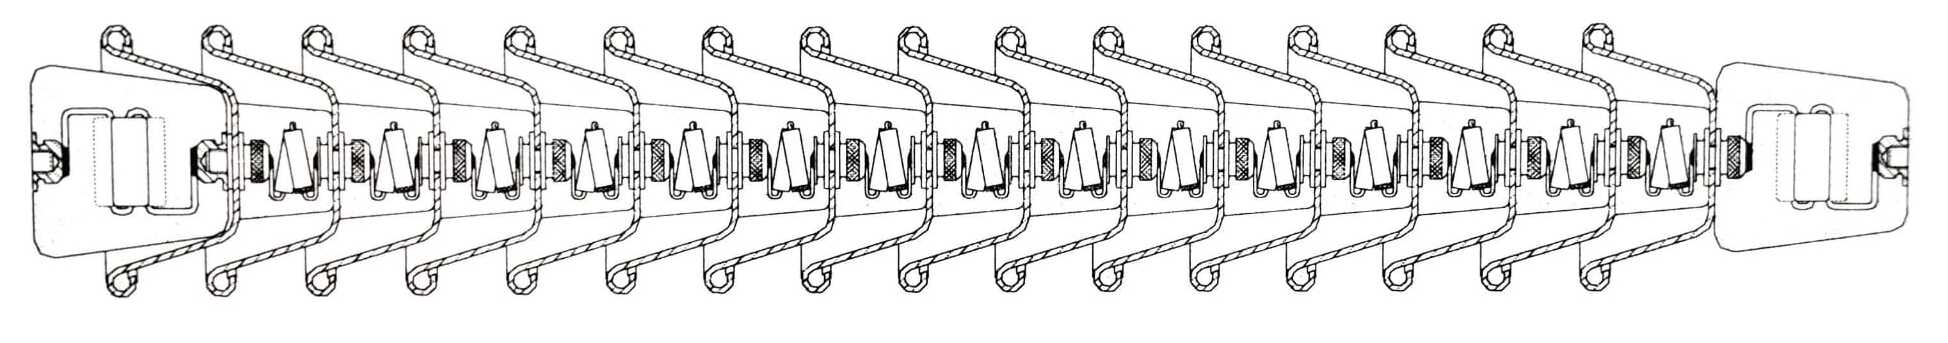
\includegraphics[width=0.8\textwidth]{Figures/MEG/CW/cw_rectifier.jpeg}\label{fig:CW:sketch:rectifier}}
            \caption{The first schematic (a) shows the CW circuit and the capacitive coupling to the RF driver while the second (b) shows the internal structure of a rectifier stack (\textit{stack ass'y}).}
        \end{figure}

        \paragraph{Driver}
        The driver, as the name suggests, is the circuit that feeds the voltage/power to the whole system.
        In between the driver and the CW stack of rectifiers' ass'ys a resonant circuit is used to amplify the output of the driver.
        The power is fed to this resonant circuit in phase with the oscillating current.
        Keeping the frequency at resonance, the driver controls the terminal voltage adjusting the pulse width.
        A block diagram of the driver is shown in Fig.~\ref{fig:CW:circuit:driver}

        \begin{figure}
            \centering
            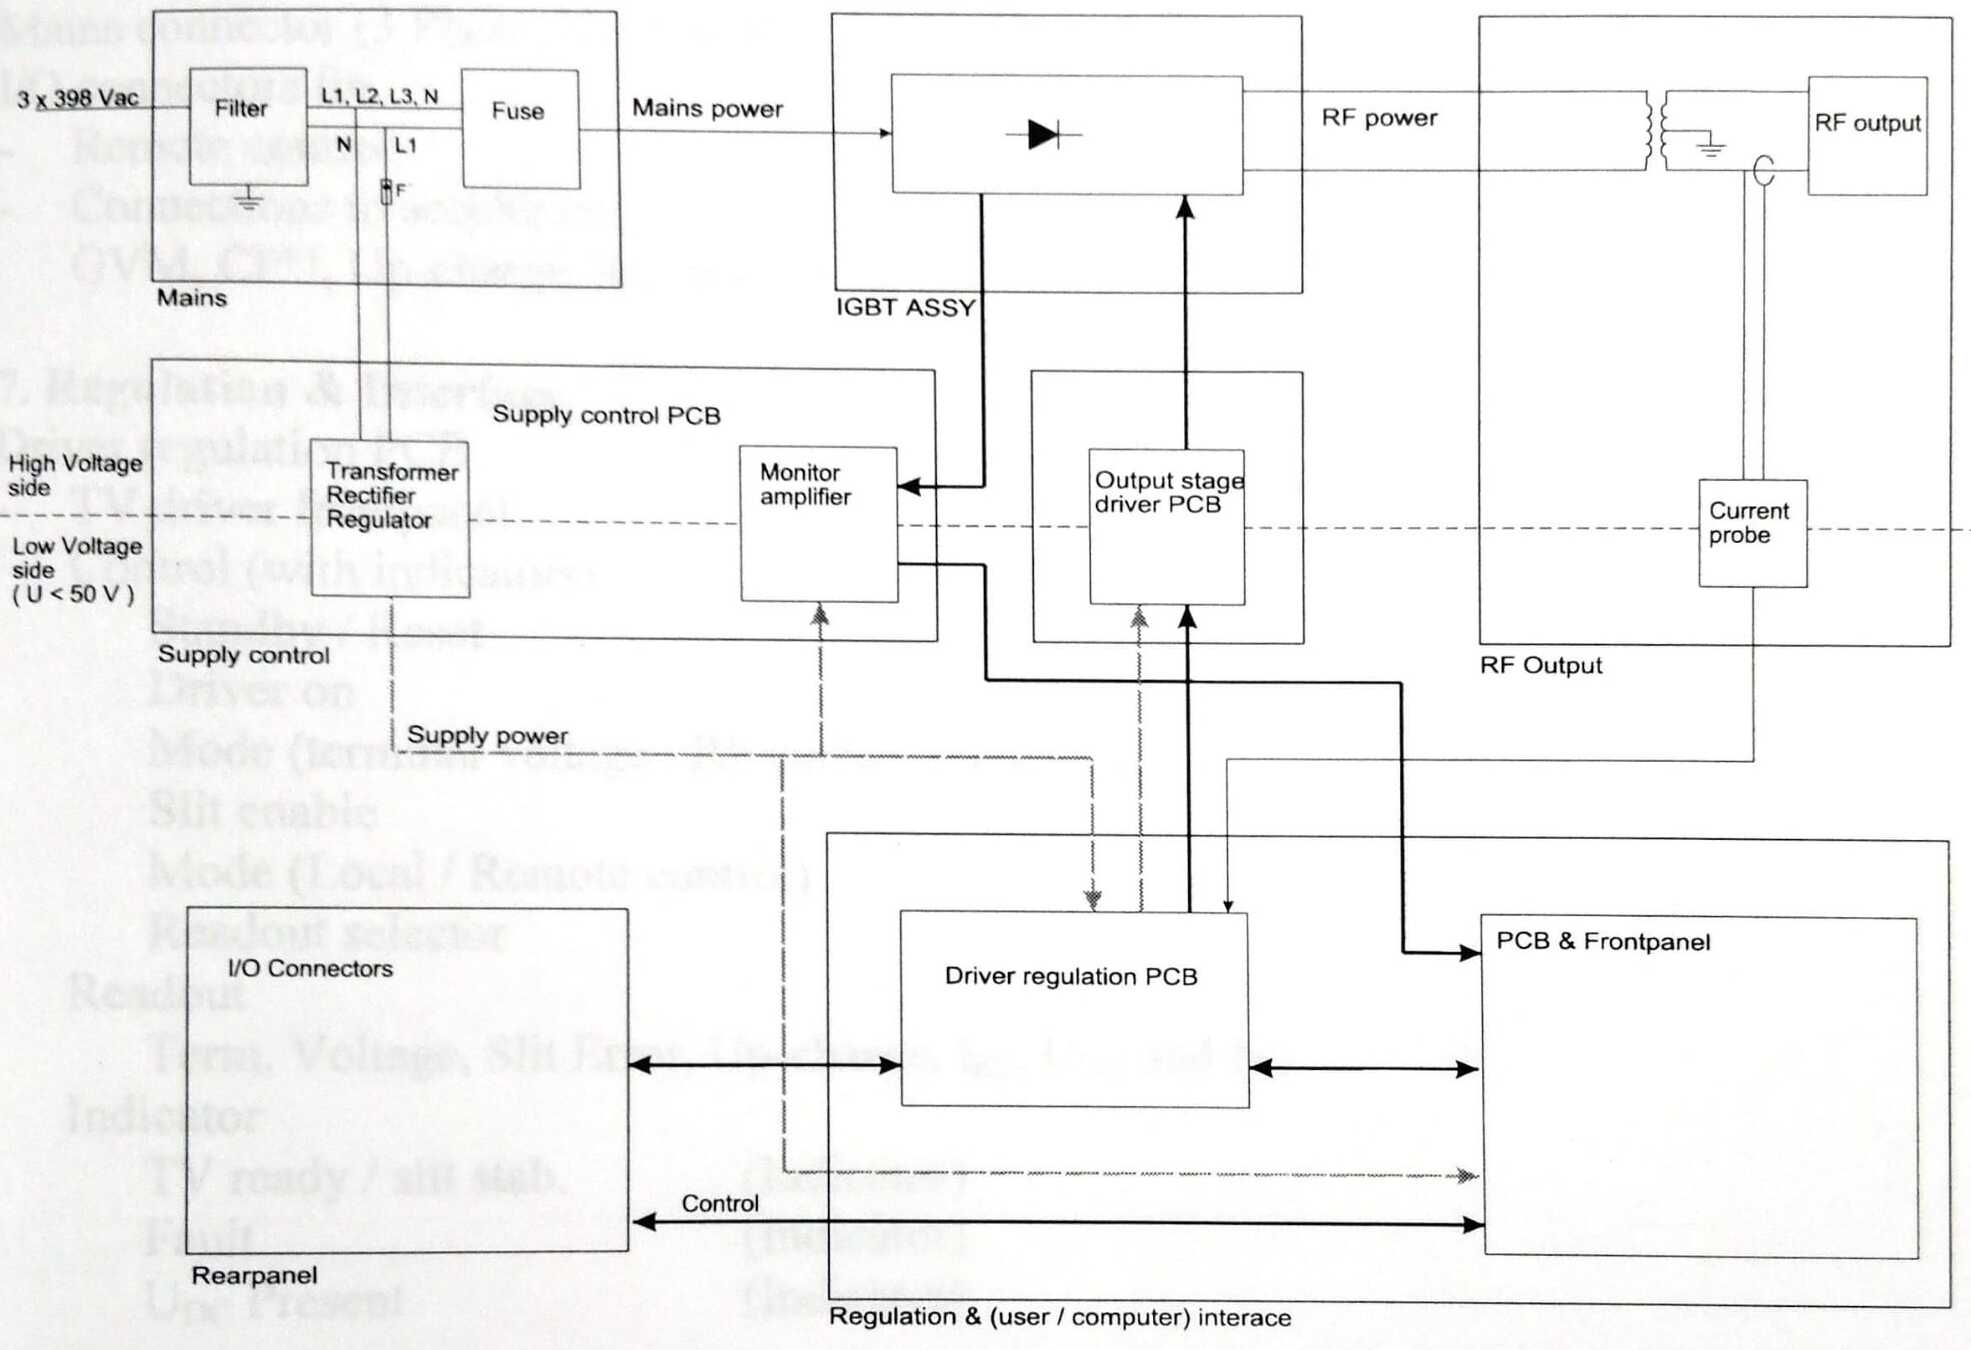
\includegraphics[width=0.8\textwidth]{Figures/MEG/CW/cw_circuit_driver.jpeg}
            \caption{Block diagram of the driver}
            \label{fig:CW:circuit:driver}
        \end{figure}

        \paragraph{Start-frequency}
        The system can operate only at resonance and this frequency $f_{res}$ is defined by the coil and dynodes.
        During star-up, the system starts at $f_{start}$ higher than the resonance and then lowers it until the resonance is found.
        A parasitic frequency $f_{par}$, with $f_{par}>f_{res}$, is also present. 
        At this frequency, the driver oscillates at a higher frequency, and no power is transferred to the terminal.
        To avoid the higher frequency, a tuning is needed so that $f_{par}>f_{start}>f_{res}$.

        
        \paragraph{Q-factor} In the RF resonance circuit high amounts of 'blind power' can be present (up to \SI{1}{MW}).
        The quality factor (Q-factor) of the RF resonance circuit is the ratio of blind to dissipated power.
        E.g. for a blind power of \SI{1}{MW} and a Q-factor of 1000 the transformer coil dissipates \SI{1}{kW} of heat.
        If this factor is not high enough the dissipated power is too high and will prevent the driver from operating correctly.
        The Q-factor is measured using a function generator and looking at the relative phase and amplitude of voltage in two points of the accelerator's RF resonance circuit.
        A sketch of the measurement is shown in Fig.~\ref{fig:CW:sketch:Q-factor}.
        The system is at resonance when there is no relative phase between $V_1$ and $V_2$, and the value of $V_1/V_2$ is used to evaluate the Q-factor: 
        \begin{equation}
            Q = Z_{coil}/R_{loss} = 2\pi f_{req} I_{coil} (V_1/V_2-1)/R_l \approx 43.9\times f_{res}[kHz]\times(V_1/V_2-1)
            \label{eq:cw:qfactor}
        \end{equation}


        \begin{figure}[ht]   
            \centering
            \subfloat[Sketch of the circuit to measure the Q-factor.]{            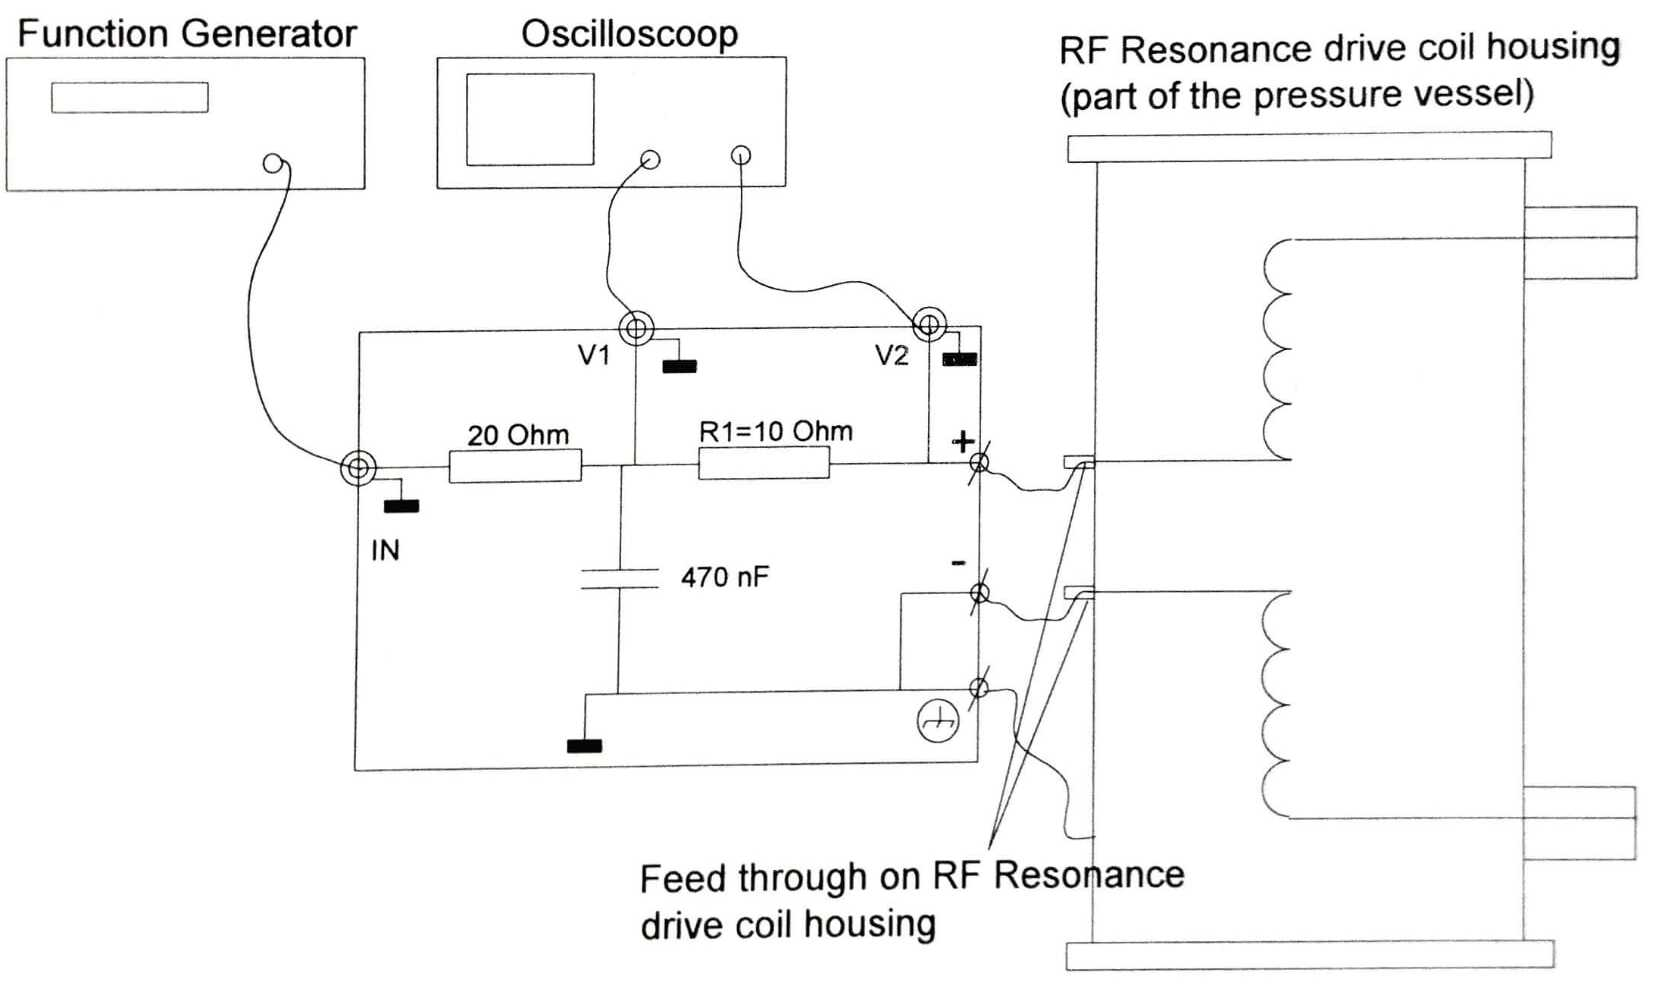
\includegraphics[width=0.49\textwidth]{Figures/MEG/CW/cw_qfactor.jpeg}\label{fig:CW:sketch:Q-factor}}
            \hfill
            \subfloat[Example of measurement of the Q-factor: in red the delay while in blue the fraction $V_1/V_2$.]{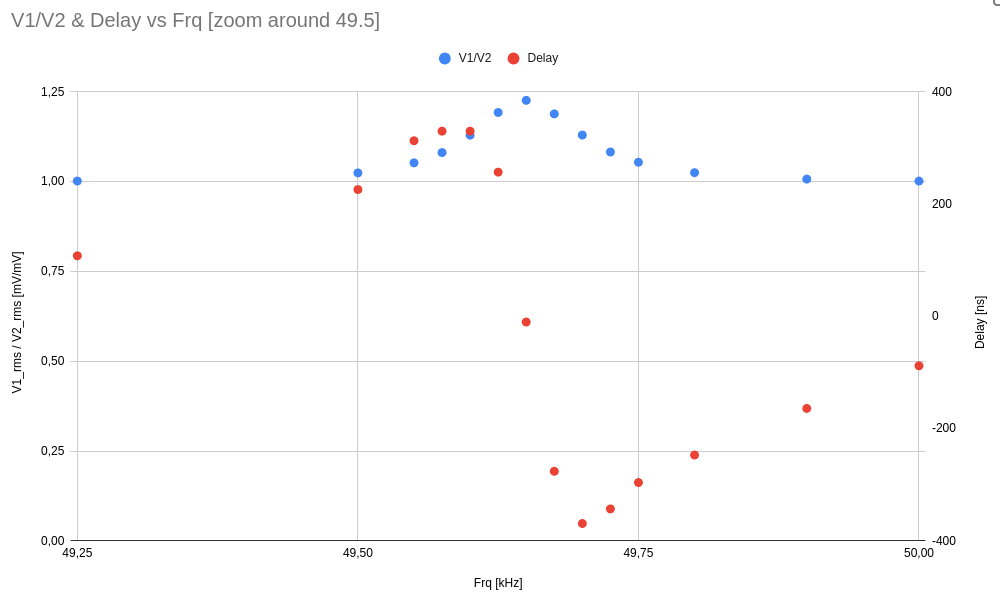
\includegraphics[width=0.49\textwidth]{Figures/MEG/CW/CW_Q-factor.png}\label{fig:CW:Q-factor}}
            \caption{The Q-factor is the ratio of blind to dissipated power. Via this number is possible to evaluate the energy dissipated as heat running the machine. If it is too low the machine cannot operate correctly.}
        \end{figure}

        \begin{figure}
            \centering
            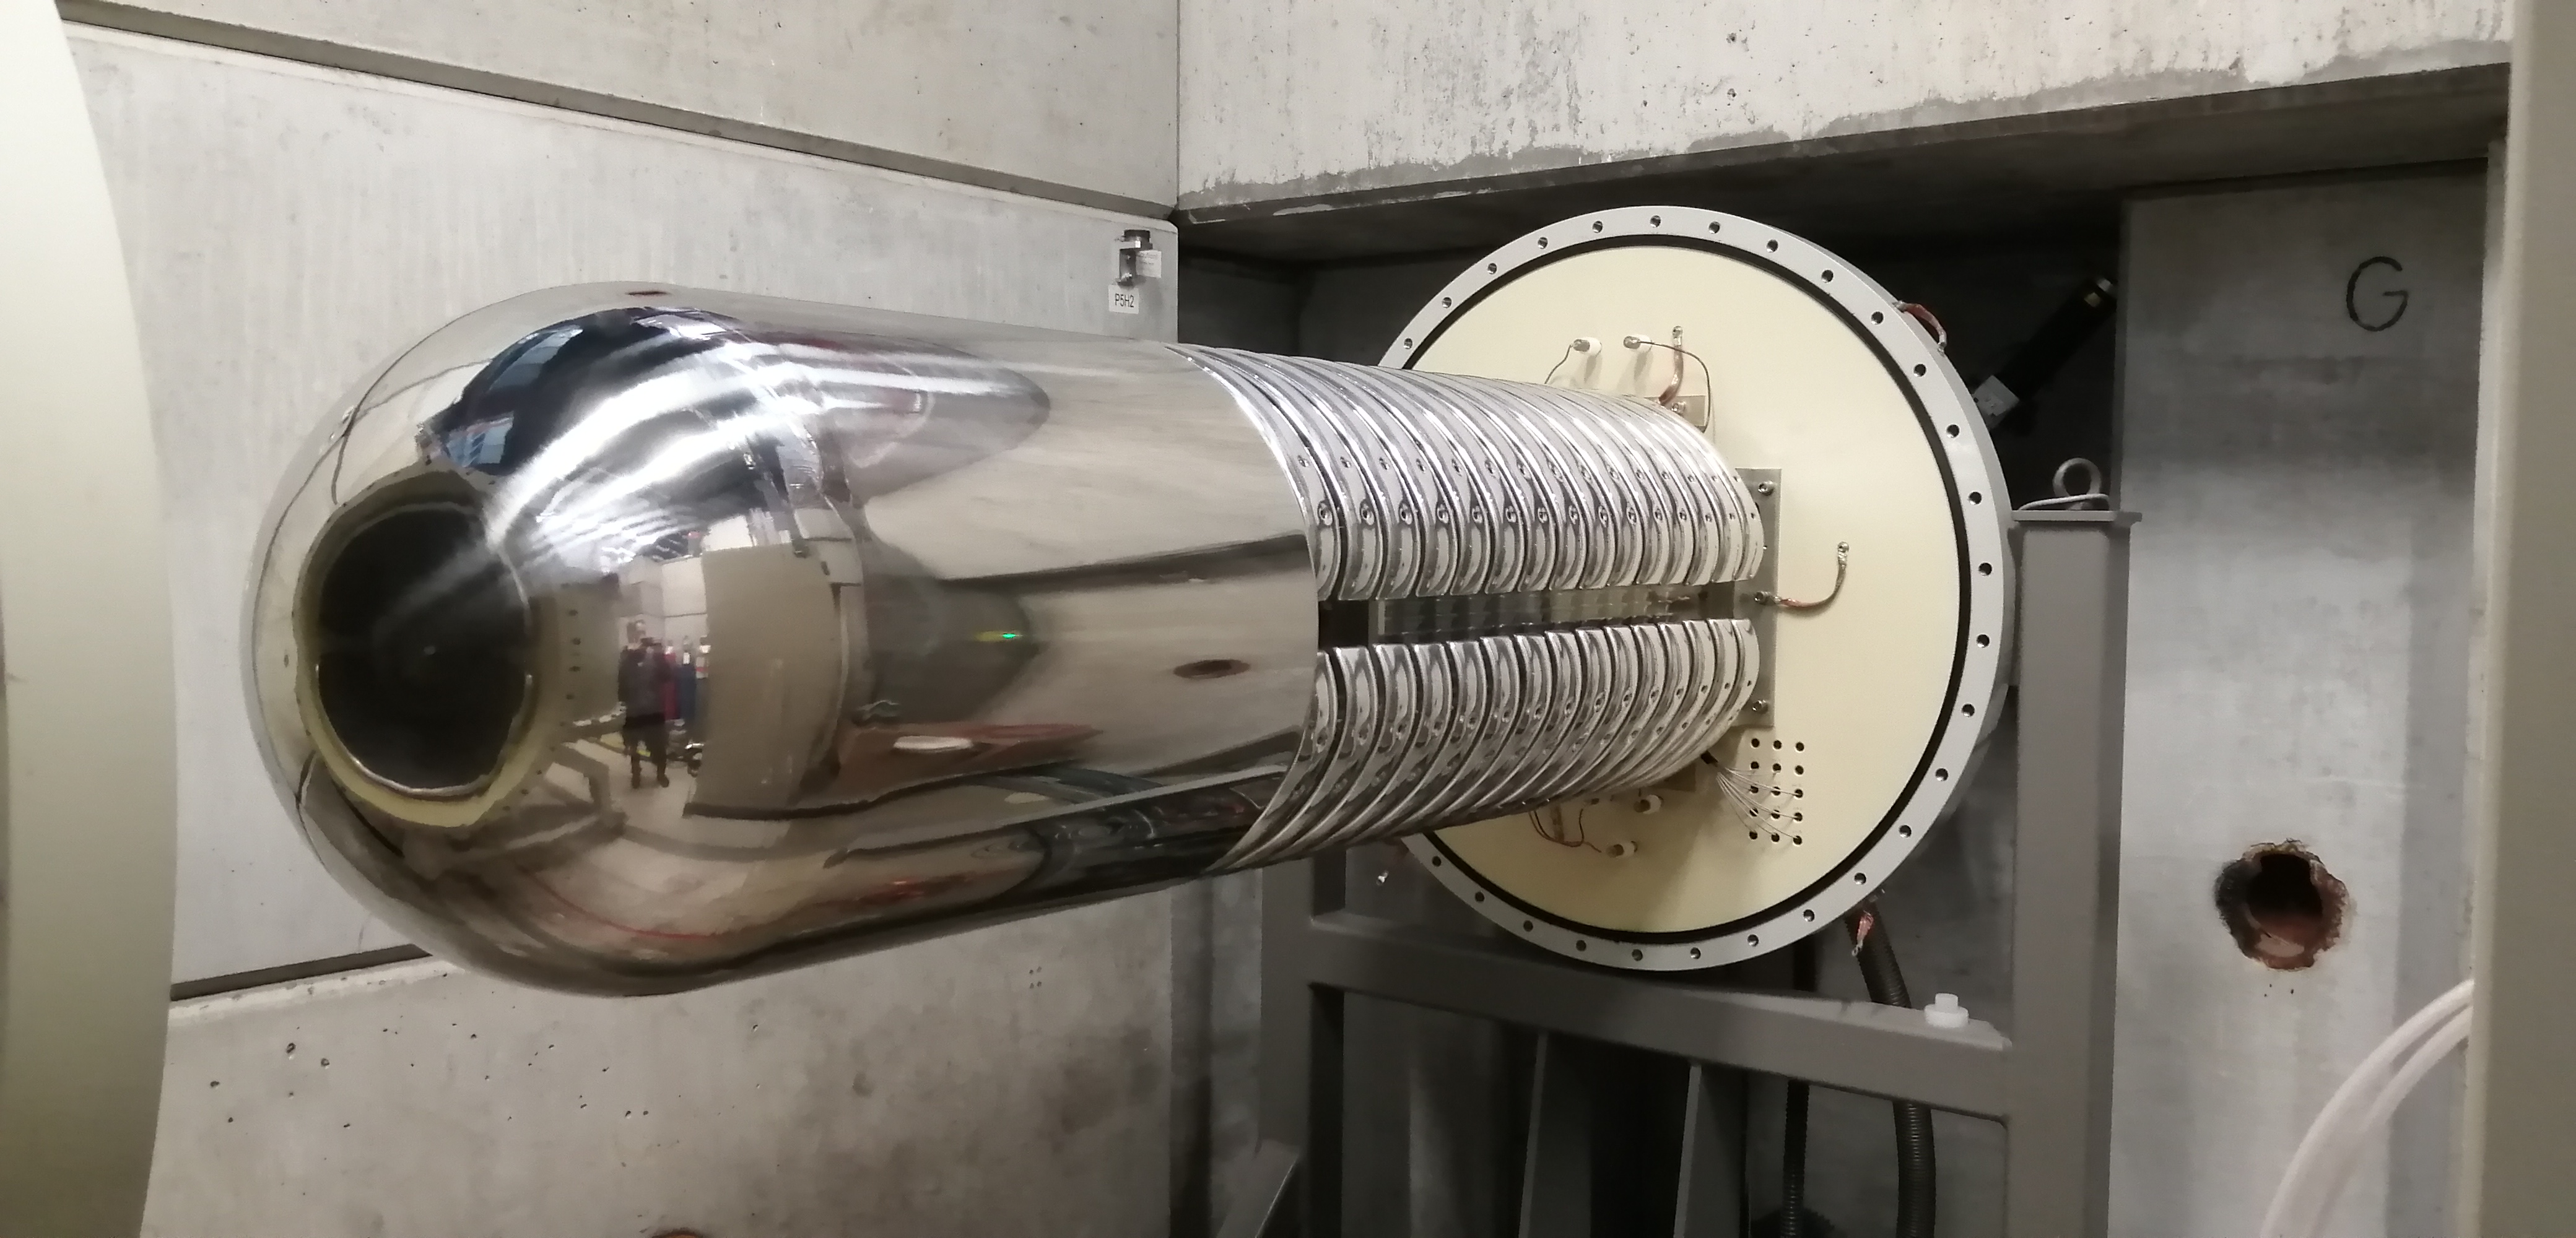
\includegraphics[width=1\textwidth]{Figures/MEG/CW/view_front.jpg}
            \caption{View of the CW after the extraction from the external volume. This volume contains \ce{SF6} which is used as a gaseous dielectric medium and needs to be evacuated before the extraction.}
            \label{fig:CW:view}
        \end{figure}

        \begin{figure}
            \centering
            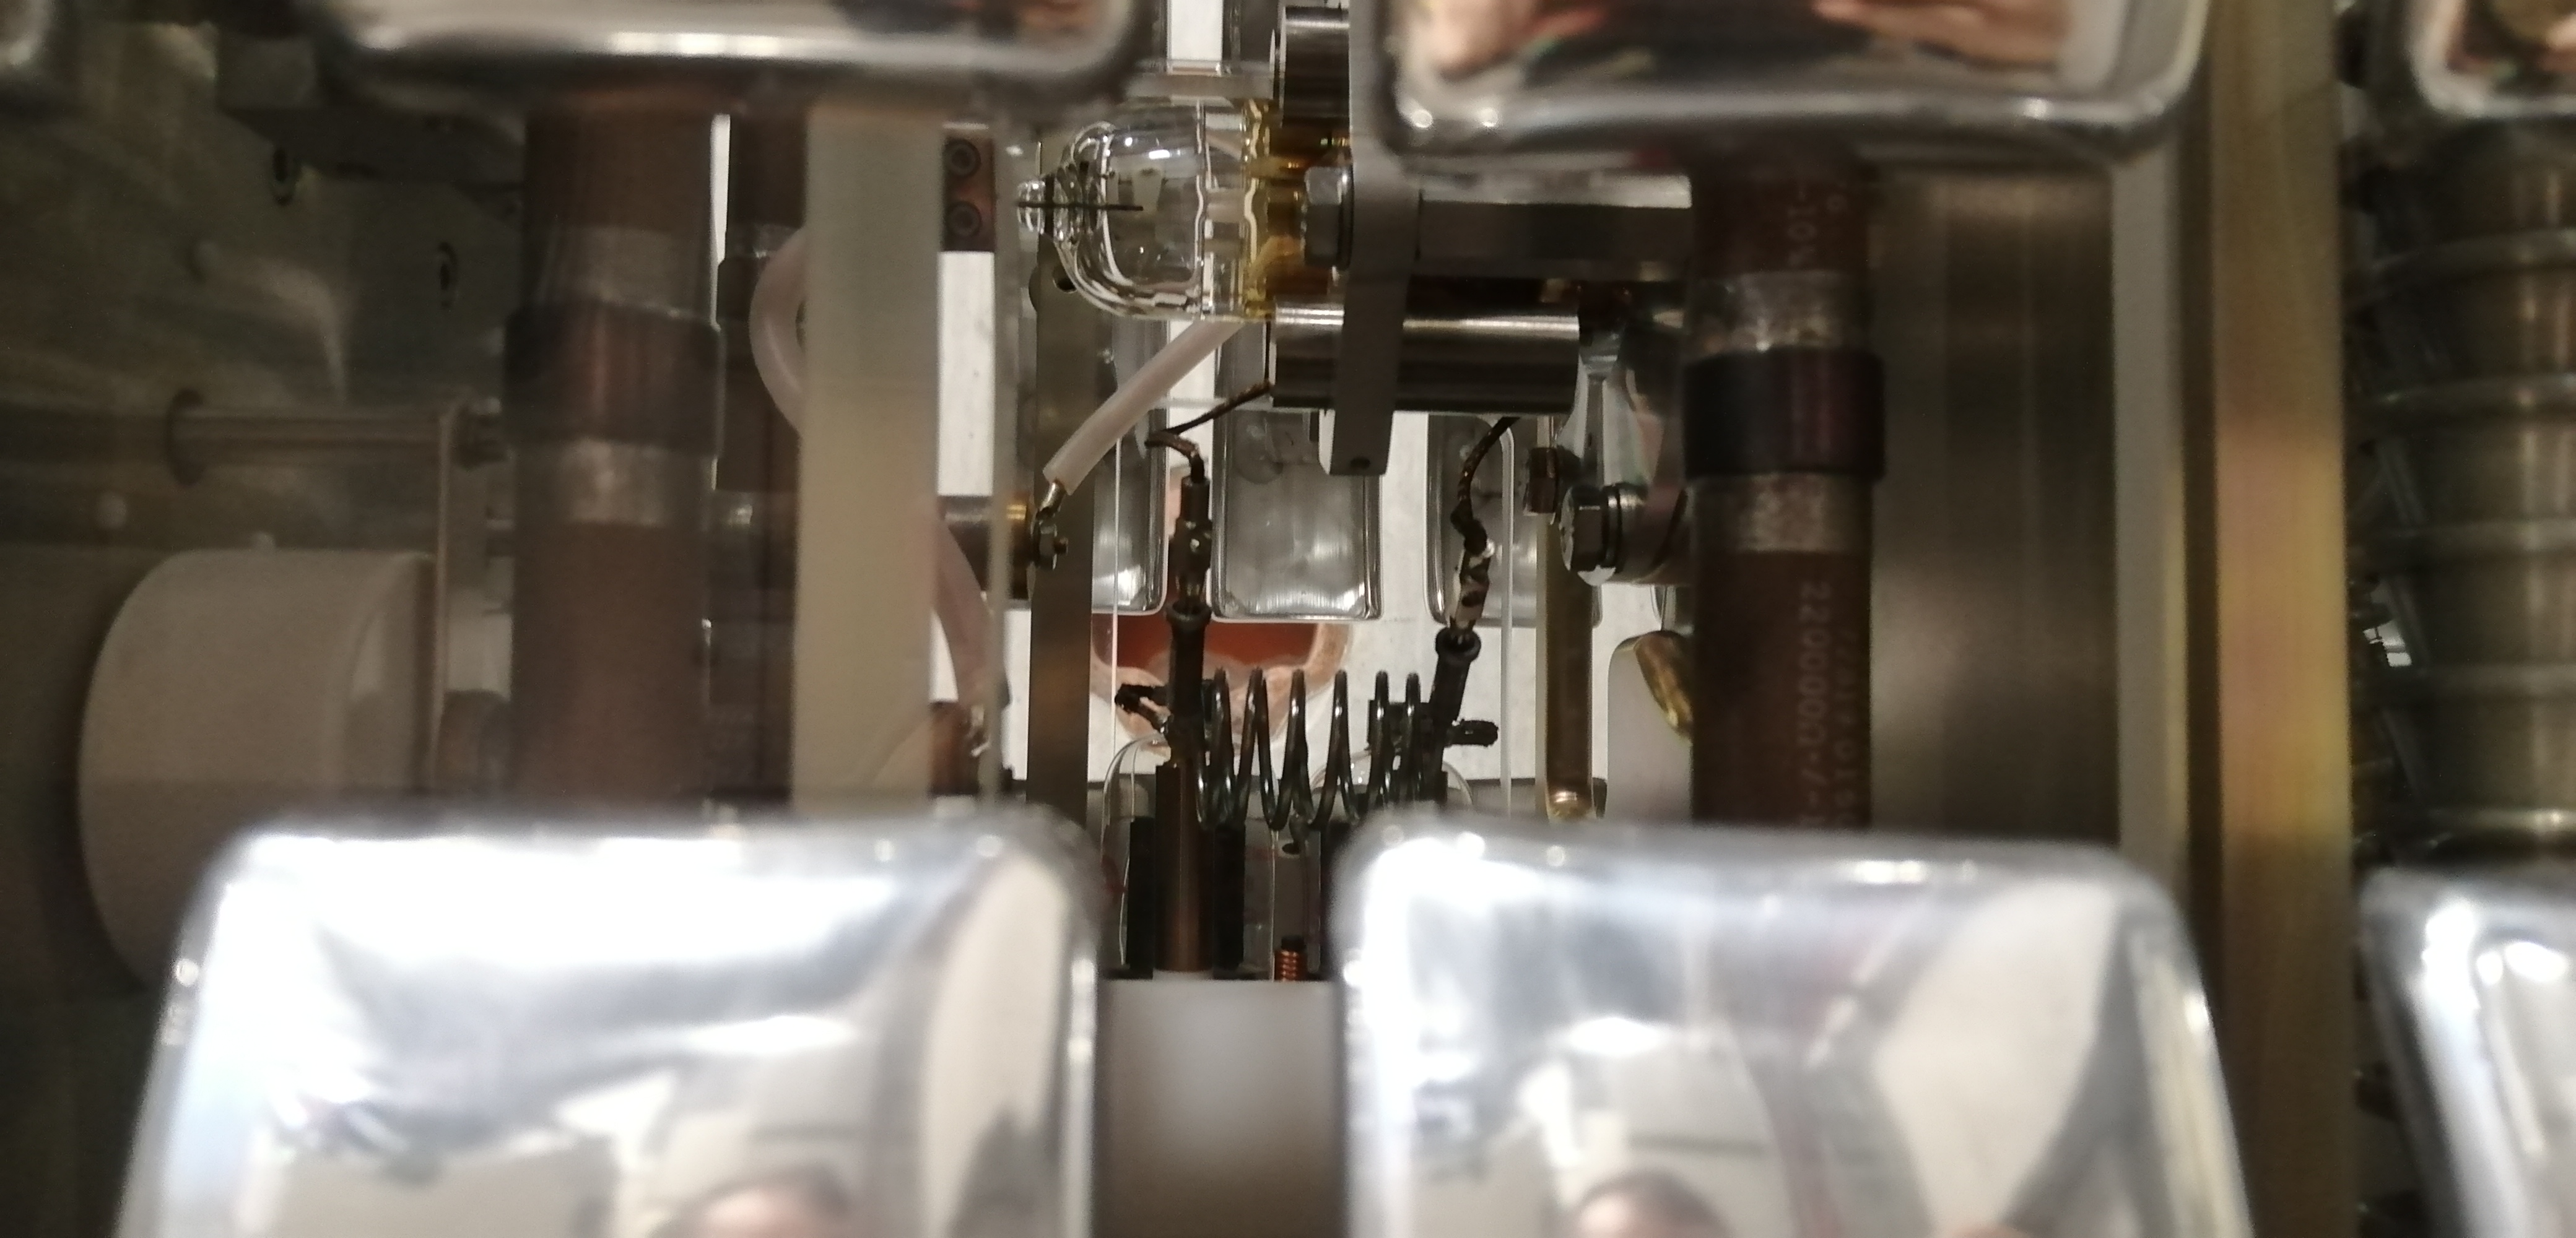
\includegraphics[width=1\textwidth]{Figures/MEG/CW/view_source.jpg}
            \caption{View of the source of the CW   machine.}
            \label{fig:CW:view_source}
        \end{figure}

        \begin{figure}
            \centering
            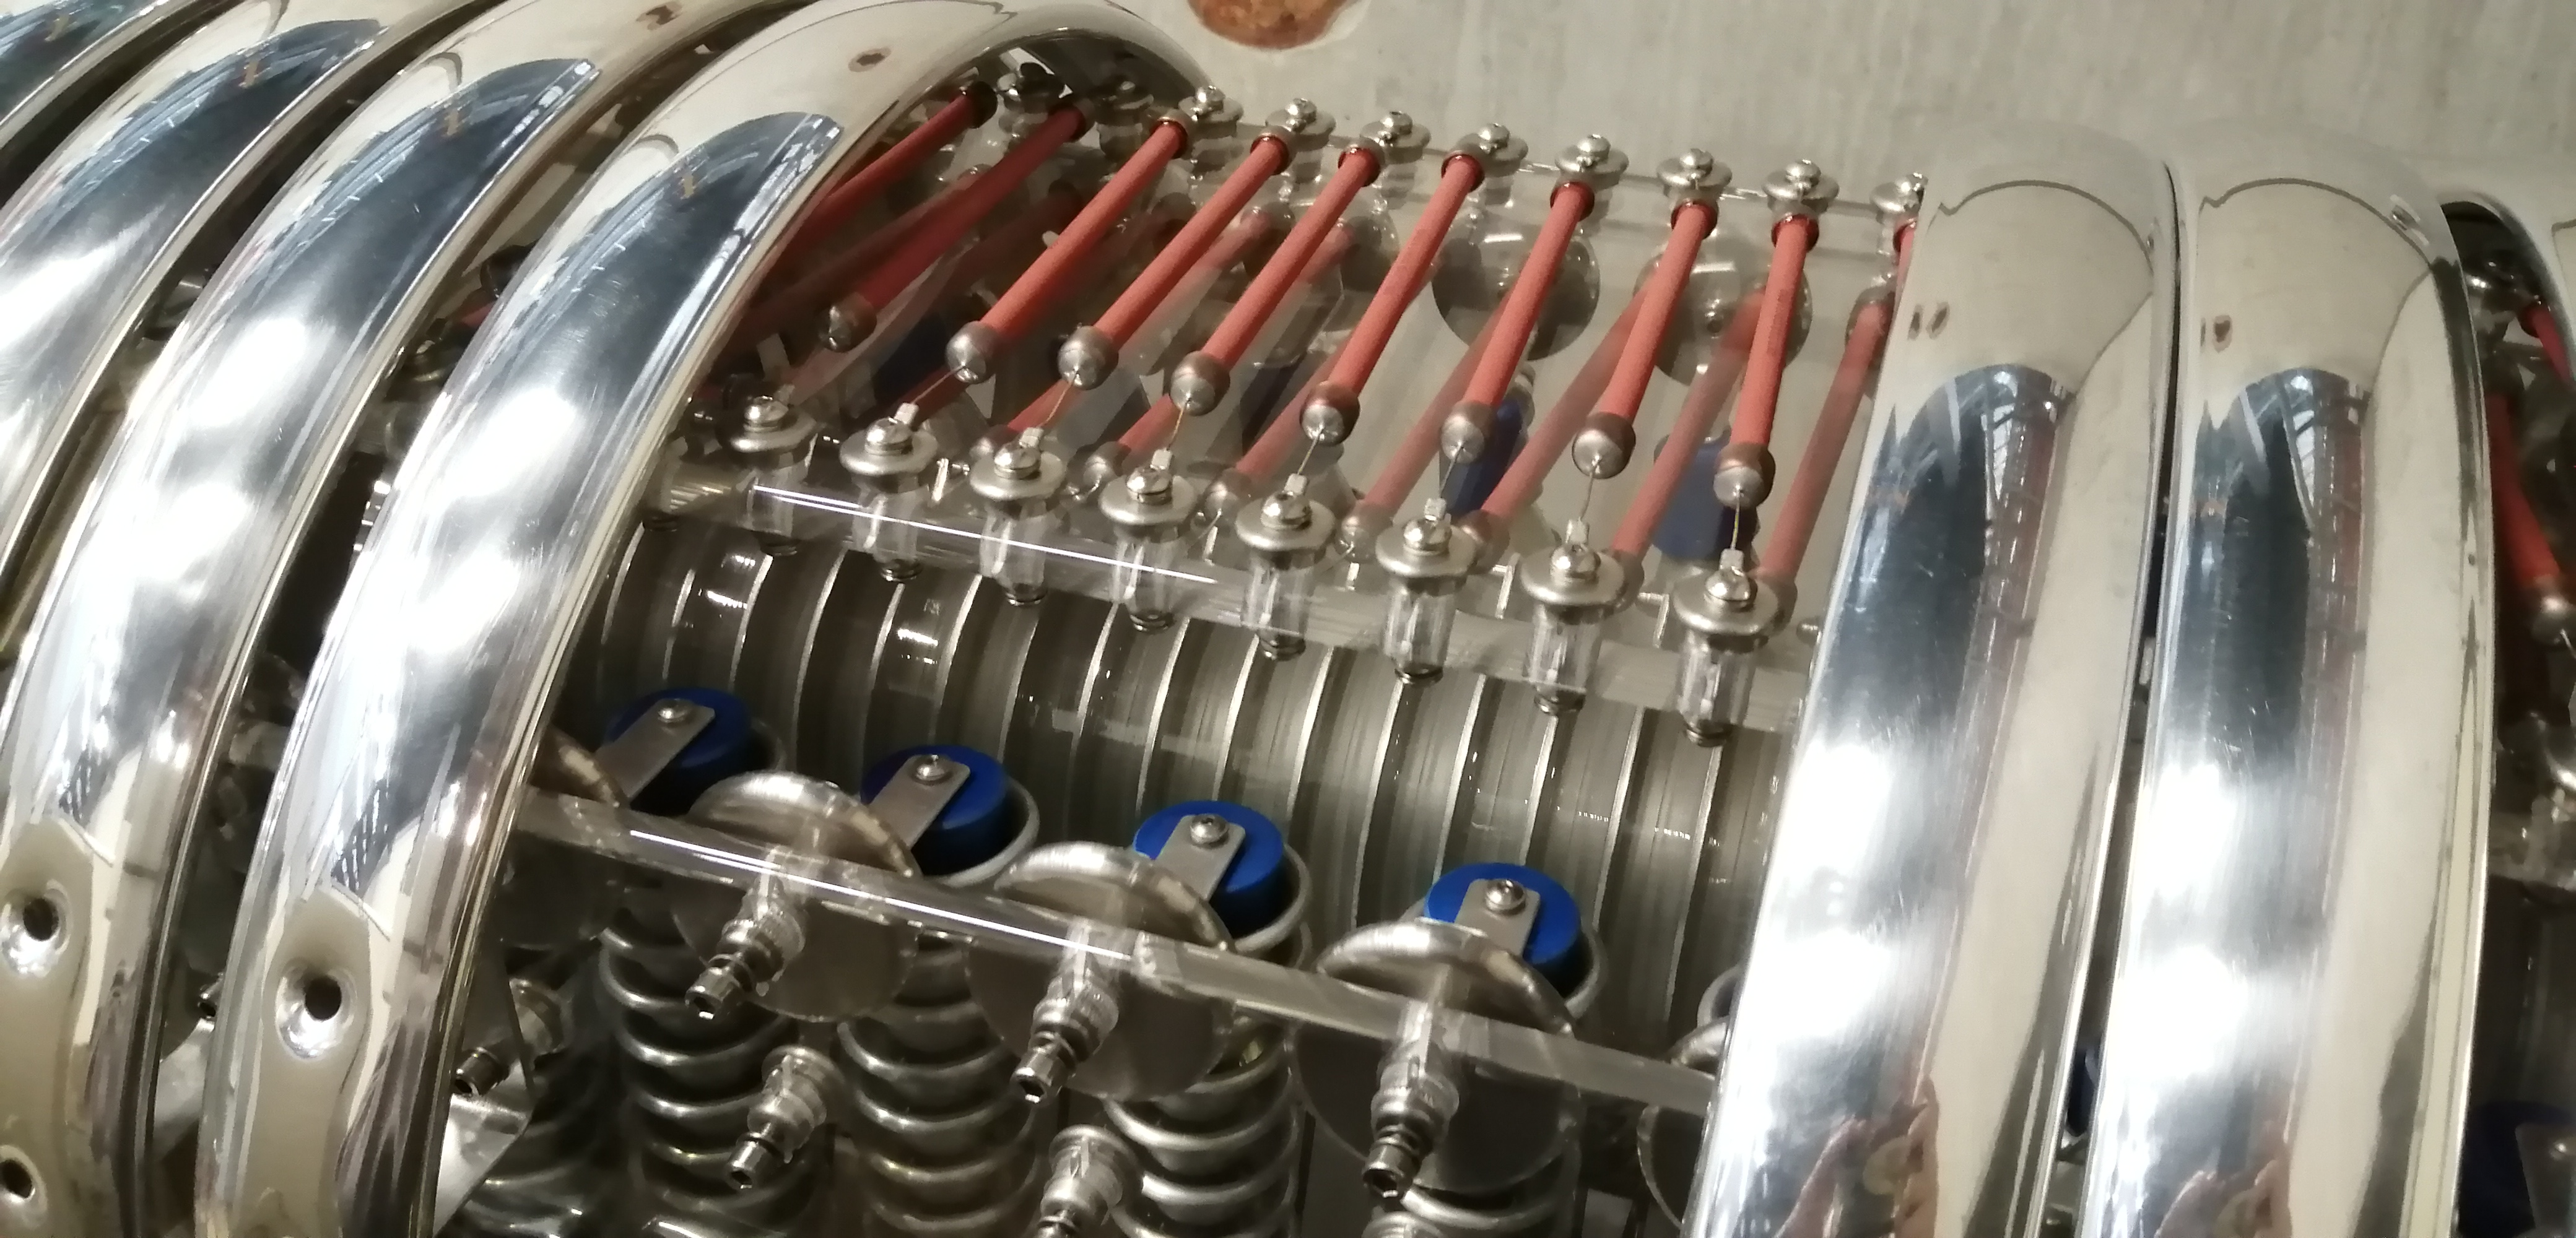
\includegraphics[width=1\textwidth]{Figures/MEG/CW/view_top.jpg}
            \caption{Top view of the CW after the removal of a few AAA. Here we can see all the elements of a CW circuit: red - the resistors on top; metallic rings on the central tube - the capacitors; blue and metallic cups - the resistance and capacitors of the rectifiers, which run vertically.}
            \label{fig:CW:view_top}
        \end{figure}

        \begin{figure}
            \centering
            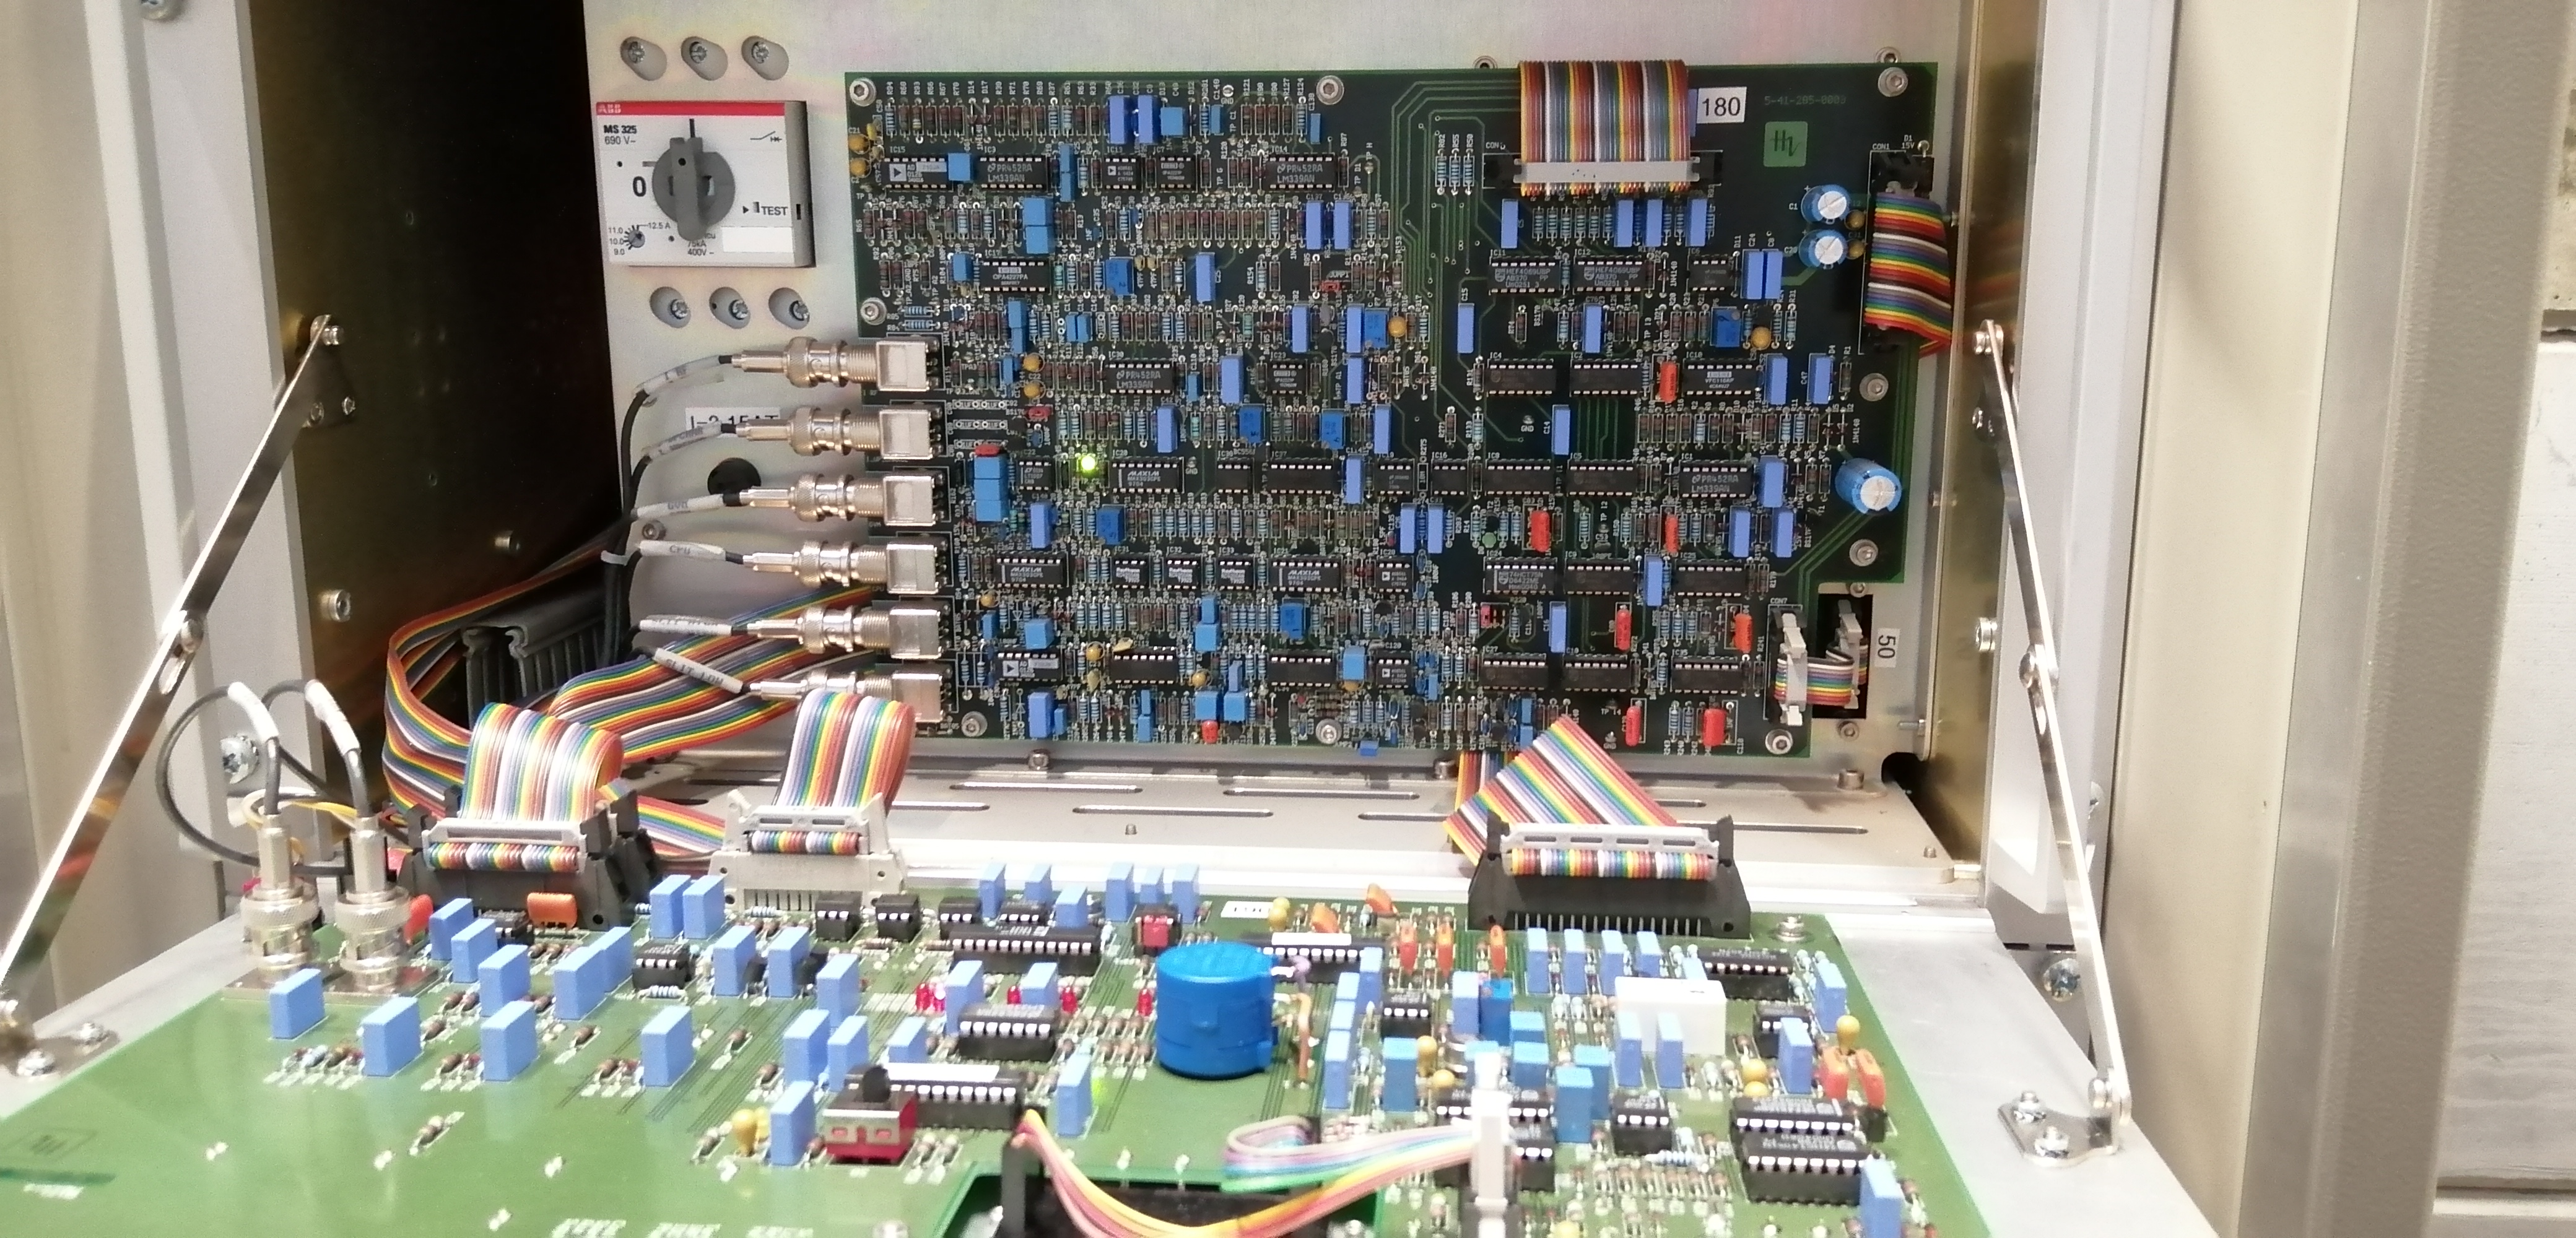
\includegraphics[width=1\textwidth]{Figures/MEG/CW/panel.jpg}
            \caption{Picture of the control panel for the CW machine.}
            \label{fig:CW:panel}
        \end{figure}

    \subsection{XEC calibrations}
        On top of the LED calibration illustrated in \ref{LED} 
        \paragraph{`Standard' lithium calibration}
        \paragraph{Charge EXchange reaction}

    \status{started}
    \subsection{X17}
        The protons coming from the CW have been mainly used for the calibration of the XEC detector, but also to perform a parasitic measurement:the search for the X17 anomaly.
        This search, done in 2021-2023, will be extensively discussed in Ch.~\ref{ch:X17} but we wanted to underline here the key role that the CW machine has played in this parasitic search for exotic physics. 

\status{review}
\section{CW issues and maintenance}
    By the end of 2020, the CW started having some minor problems: the machine was running fine but the time required to switch it on kept growing longer. 
    While the whole procedure would normally take $\sim$ 15 min the time required exceeded the hour.
    We also noticed the machine was getting unstable when running near the maximum voltage at \SI{1}{MV}.
    Following this behavior, an intense exchange with the HVEE company started and we performed many different tests on both the software and hardware sides.
    
    \paragraph{Hot Fix}
    We performed a measurement of the Q-factor of the machine using Eq.~\ref{eq:cw:qfactor}, shown in Fig. \ref{fig:CW:Q-factor}.  
    The value found was a factor $\sim2k$ lower than expected and the position of the resonance frequency was shifted from the design value.
    For more information on the functioning of the machine and the Q-factor see Sec.~\ref{sec:cw:machine}.
    We adjusted the frequency at which the machine starts when turning ON. 
    This solved the delay problem but didn't recover the maximum voltage. \\
    The machine was now starting quickly but working in a stable configuration only up to half of the nominal maximum voltage.
    As explained in the previous paragraph this was not a problem for the `usual' calibrations but was a worrying sign on the health of the machine and would have prevented the CEX.
    At this point, an expert from HVEE was sent to inspect the machine.

    \paragraph{Proper Fix}
    After running some checks opening the CW was deemed necessary and for this reason, we removed the \ce{SF6} contained in the main tank. 
    After the extraction of the CW, we inspected and measured all the elements, removing also some of the \textit{corona rings} for easier inspection. 
    We found signs of arcing on one of the \textit{rectifier ass'y}. 
    After the substitution of this element\footnote{The rectifier ass'y are stacks of alternated diodes and aluminum capacitors capped by two resistors. We could re-use the capacitors, after careful cleaning, while resistors and diodes were too badly damaged. The process of refurbishing is shown in Fig.~\ref{fig:CW:fixed}}, the machine was closed again, filled with \ce{SF6}, and tested again.
    This whole process is shown in the pictures in Fig.~\ref{fig:CW:broken}.
    Unfortunately, the faulty behavior persisted and we noticed sparks in the main volume. 
    After re-opening we found burning marks on the rectifier ass'y next to the exchanged one.
    We then realized that both were damaged but the first was functioning as a `bridge', preventing the second from being completely destroyed. 
    After the substitution of the second and the tuning of the machine, we finally recovered its full functionality: quick switching ON and stable operation in the full range of voltages.
    \ref{fig:CW:fixed}.

    \begin{figure}[ht]   
        \centering
        \subfloat[Discovery of the burning marks on two rectifiers. The reflectivity was a challenge in taking the picture.]{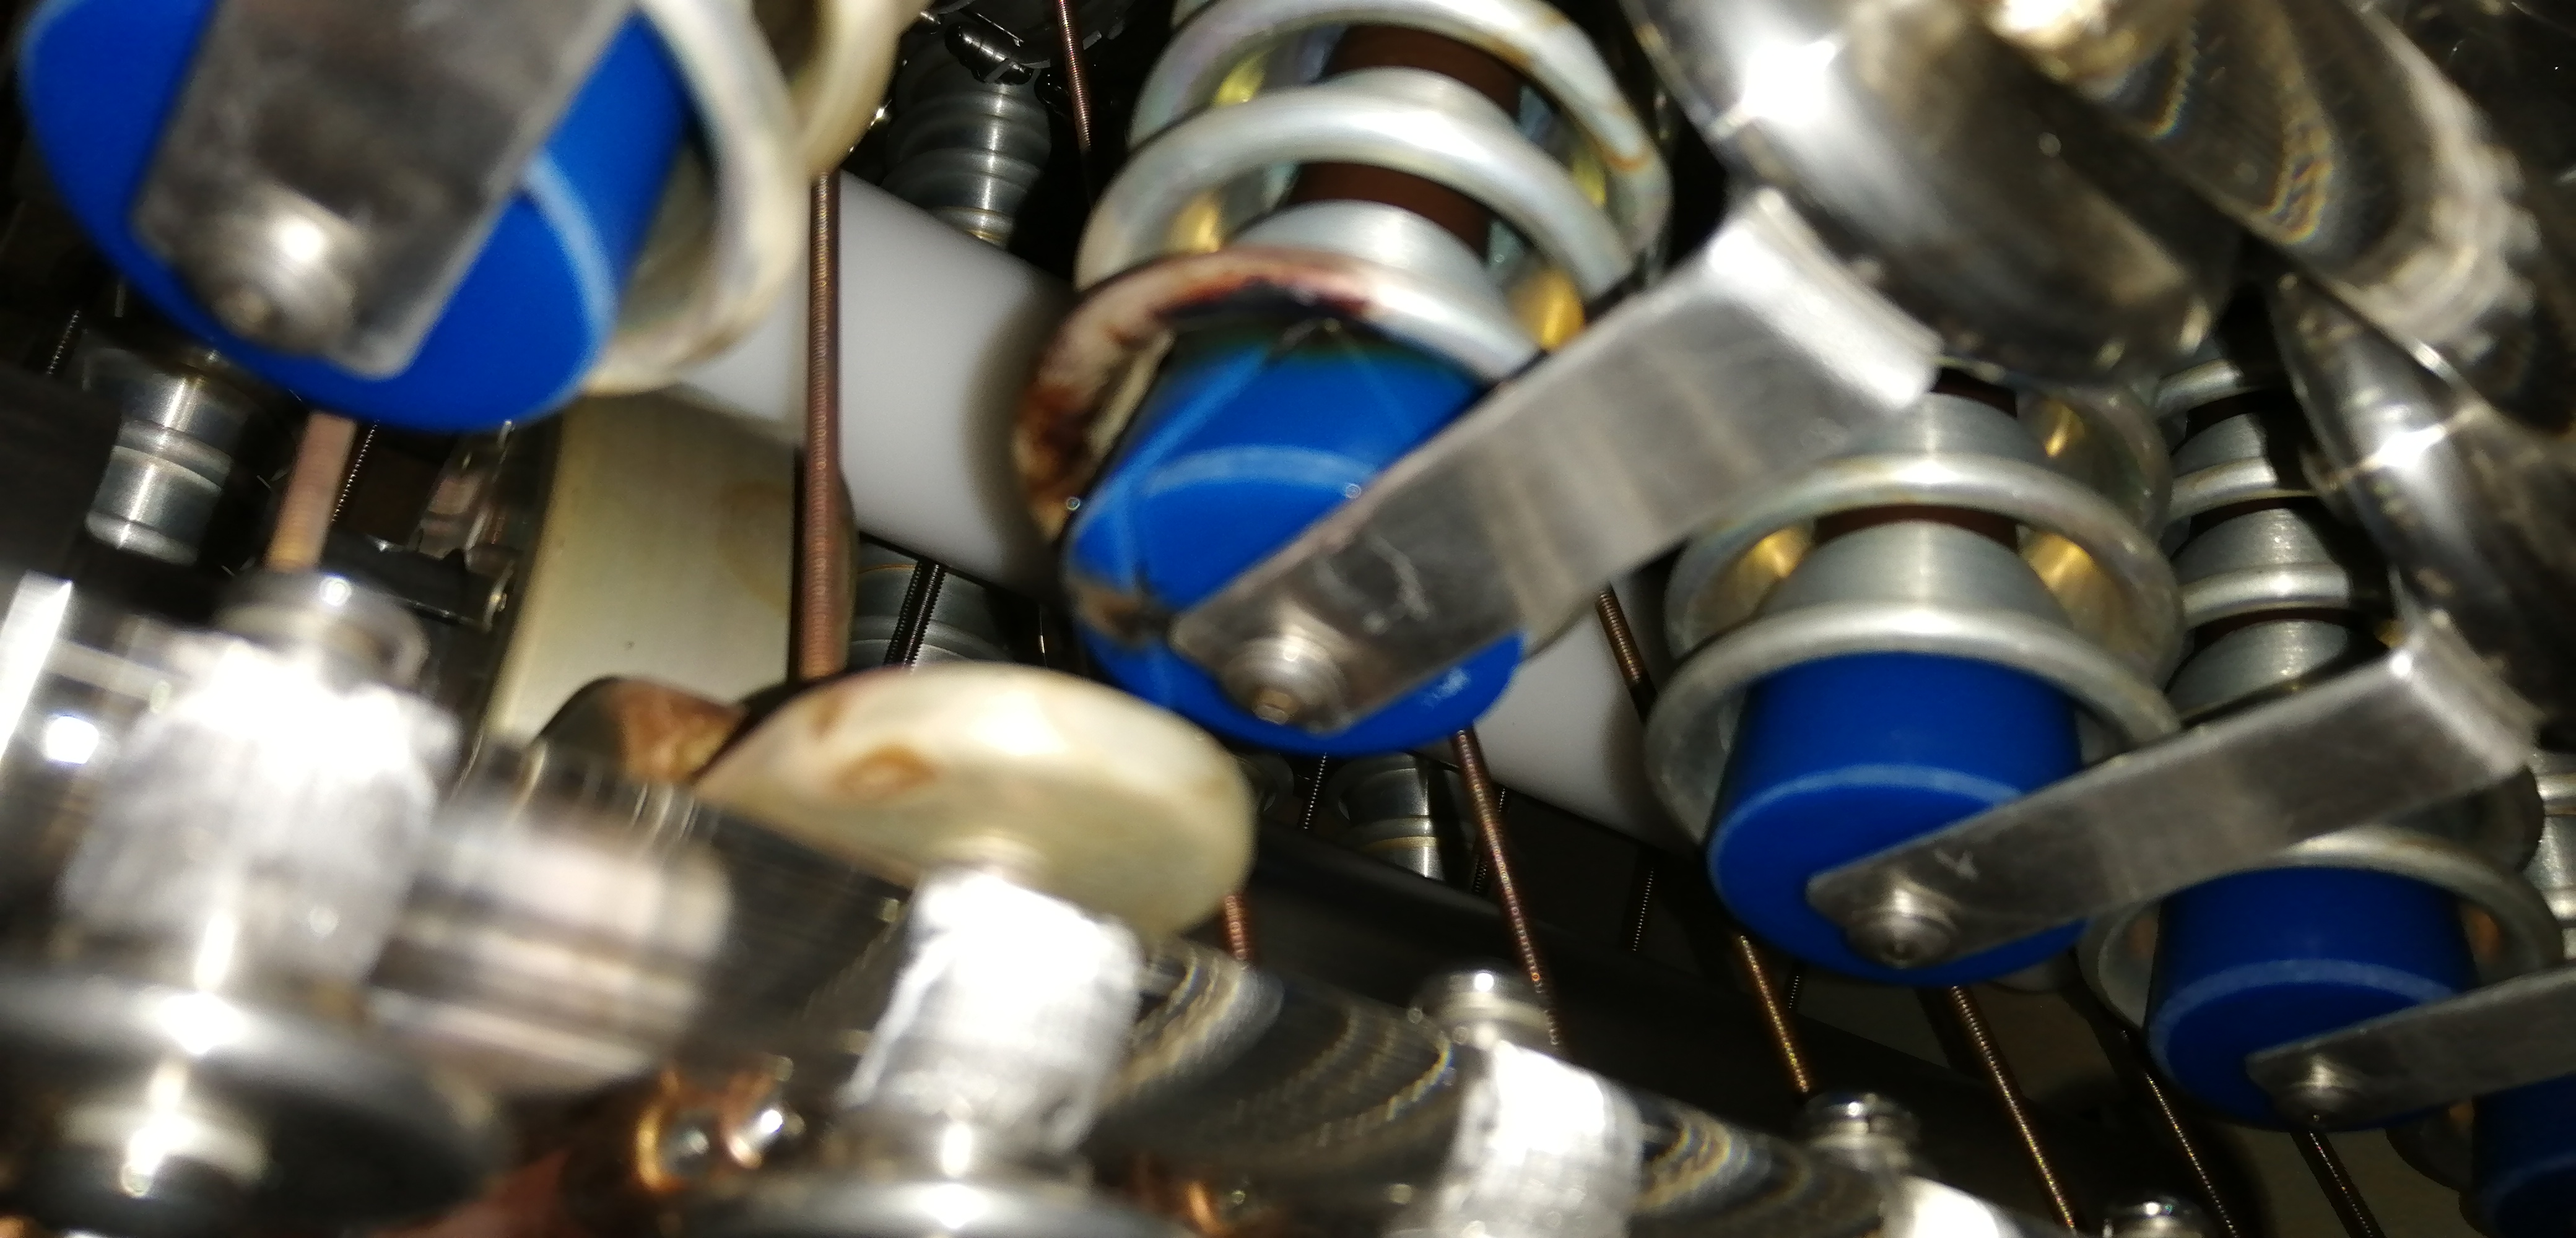
\includegraphics[width=1\textwidth, keepaspectratio]{Figures/MEG/CW/bnurned_in.jpg}\label{fig:CW:burned_in}}\\
        \subfloat[Extraction of the broken rectifiers.]{
        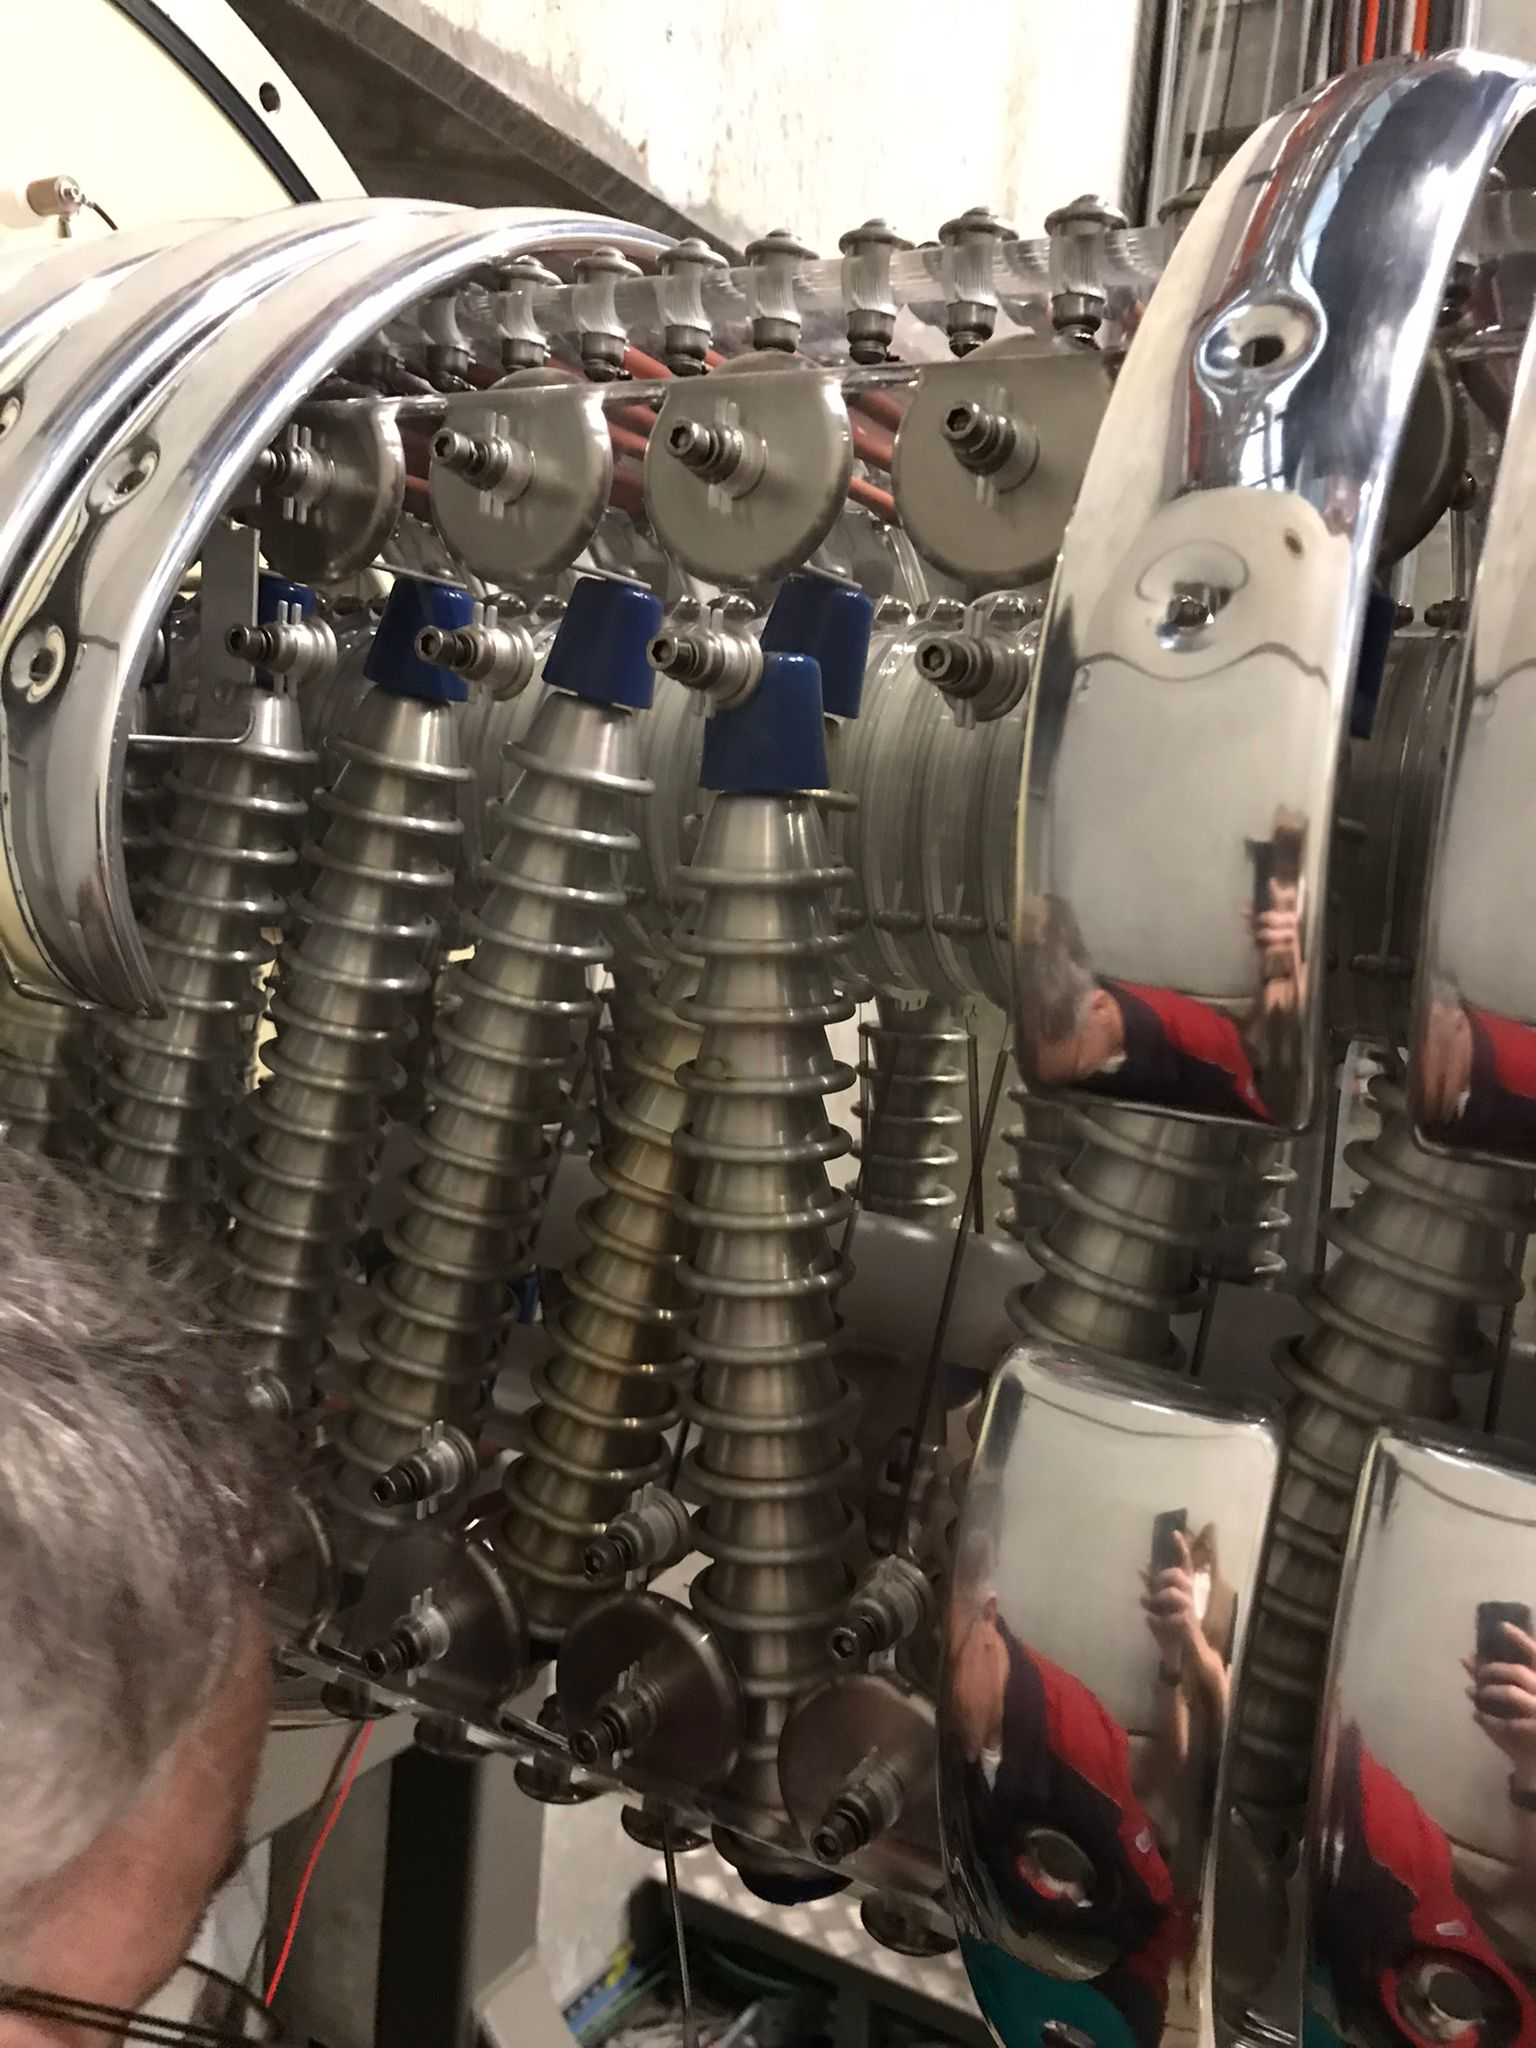
\includegraphics[width=0.49\textwidth, keepaspectratio]{Figures/MEG/CW/removal.jpg}\label{fig:CW:removal}}
        \hfill
        \subfloat[Broken rectifier ass'y after the extraction: clearly visible is the burned blue resistor at the top.]{
        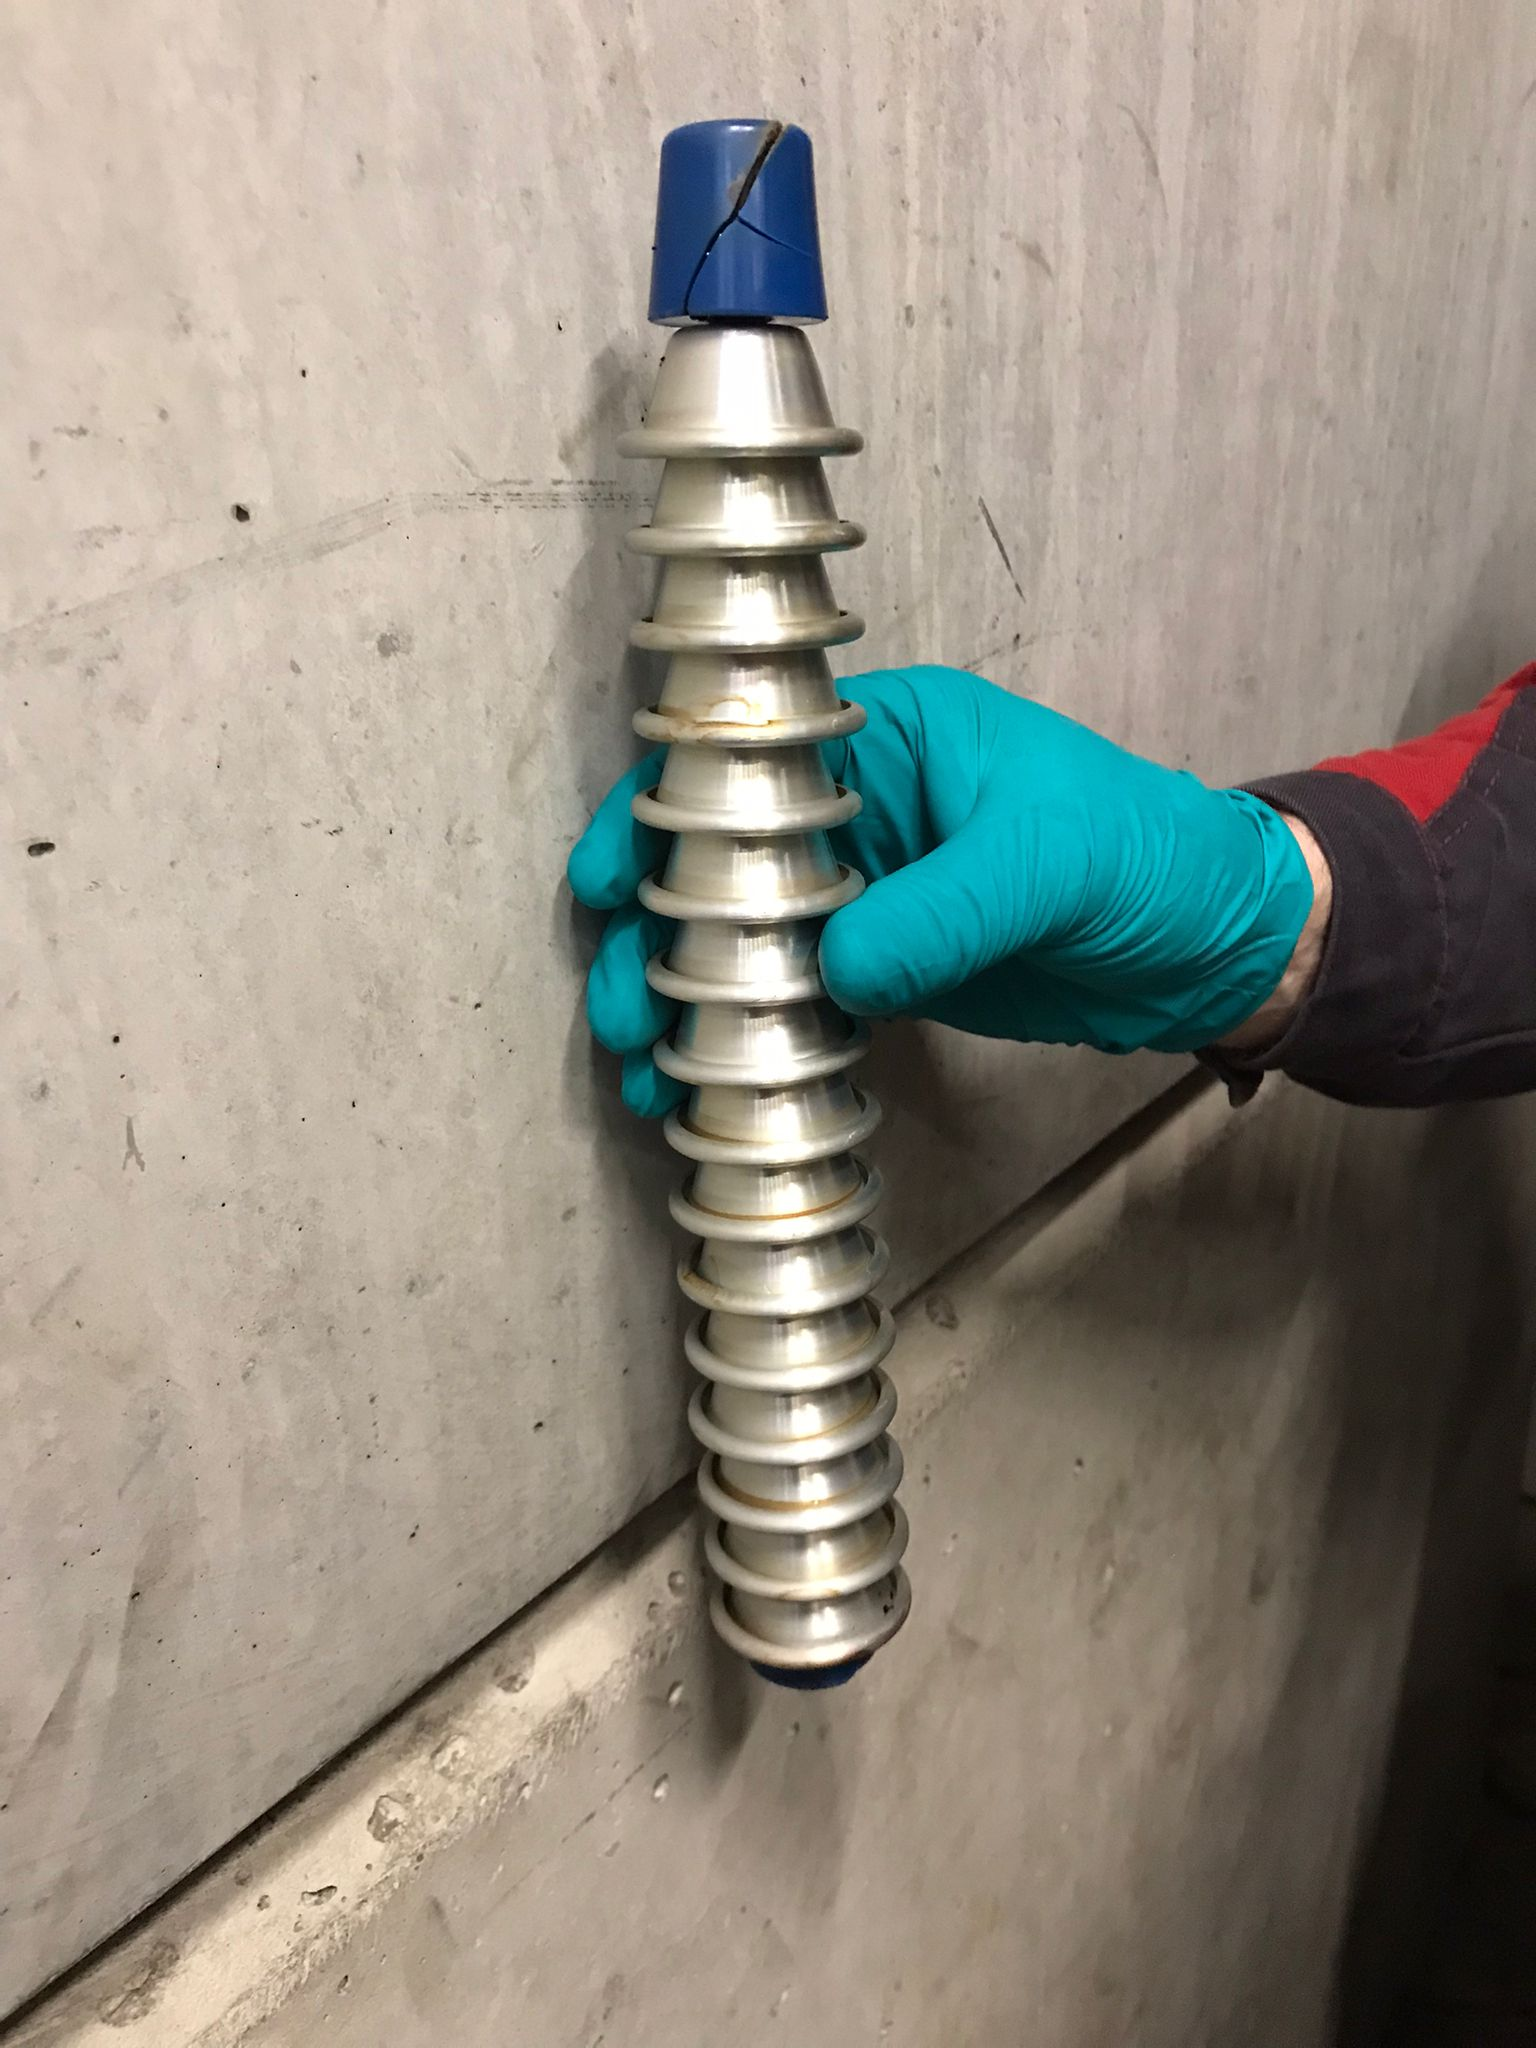
\includegraphics[width=0.49\textwidth, keepaspectratio]{Figures/MEG/CW/rect_broken.jpg}\label{fig:CW:rect_broken}}
        \caption{After close inspection we found burning marks on two rectifiers' ass'y (\ref{fig:CW:burned_in}). These were removed (\ref{fig:CW:removal}) and carefully inspected (\ref{fig:CW:rect_broken}). The only salvageable part of the rectifiers were the aluminum capacitors, which we cleaned from burning residuals, while all diodes and resistors had to be exchanged.}
        \label{fig:CW:broken}
    \end{figure}

    \begin{figure}[ht]   
        \centering
        \subfloat[Picture of the burning marks on the end resistors of the rectifier ass'y.]{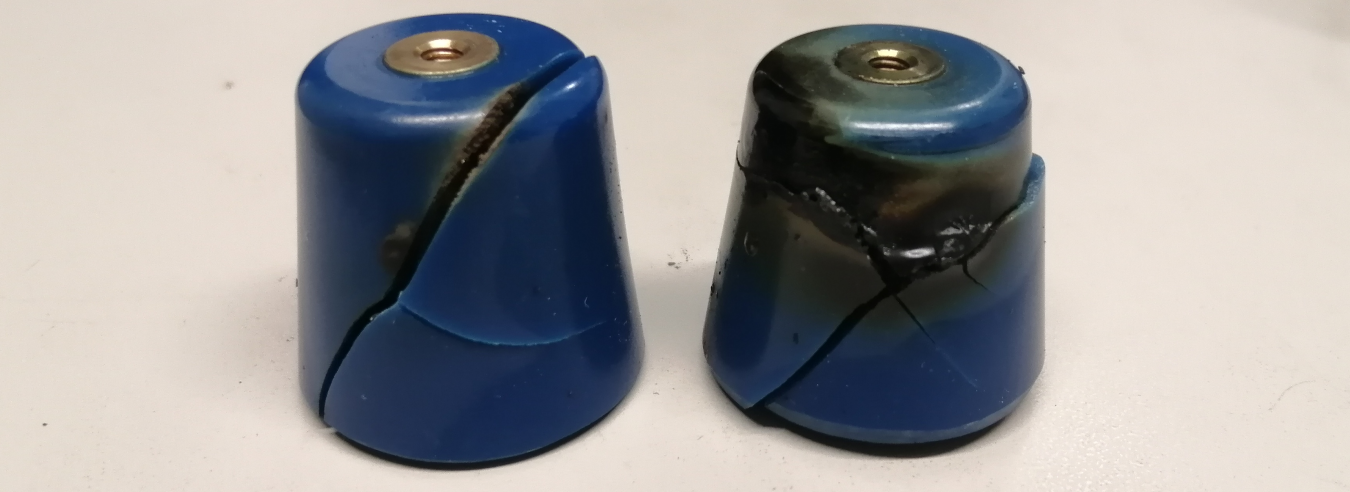
\includegraphics[width=1\textwidth, keepaspectratio]{Figures/MEG/CW/burned.png}\label{fig:CW:burned}}\\
        \subfloat[Assembly of one of the new stack: black - resistors; brown - diodes; metallic - aluminum capacitors.]{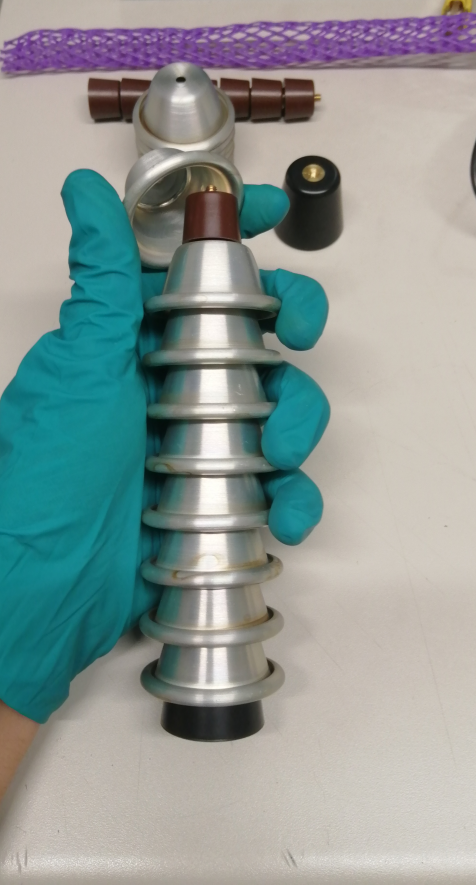
\includegraphics[width=0.49\textwidth]{Figures/MEG/CW/rect_build.png}\label{fig:CW:rect_build}}
        \hfill
        \subfloat[One of the finished new rectifiers.]{       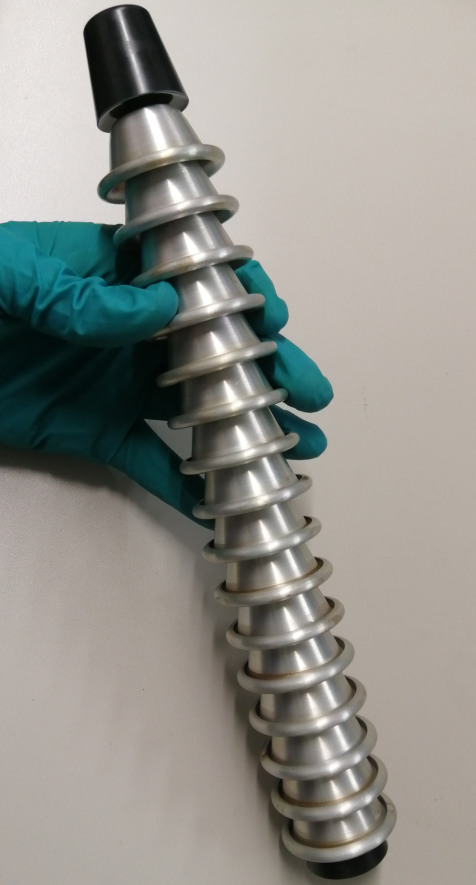
\includegraphics[width=0.49\textwidth, keepaspectratio]{Figures/MEG/CW/rect_new.png}\label{fig:CW:rect_new}}
        \caption{The rectifiers are made of three elements: diodes; aluminum capacitors; resistors (\ref{fig:CW:burned}). Only the capacitors were salvageable: we re-assembled the rectifiers with new diodes and resistors (\ref{fig:CW:rect_build}; \ref{fig:CW:rect_new}).}
        \label{fig:CW:fixed}
    \end{figure}

\status{started}
\section{Conclusions}
In this (very dense) chapter we went through the description of two key elements of the work I have done during these three years: the MEG II apparatus and the Cockcroft–Walton.
While I took no part in the design of either, in these years I spent a lot of time `hands-on' on many subsystems of the MEG II apparatus: calibrations, tuning, and fixes of various types.
On the other side, the CW functioning has been one of my main tasks.
The unfortunate hiccup with the CW gave me the additional unforeseen opportunity to assist the HVEE technician in testing and fixing the machine, which was an extremely interesting experience. 

\status{started}
\printbibliography[
    heading = bibliographychapter,
    title=Bibliography on MEG II
]

\end{refsection}
